\chapter{Web Server}
Analizzare le performance di un web server Apache, effettuando le seguenti attività:

\begin{itemize}
    \item \textbf{Capacity Test:} Valutazione delle performance del sistema al ariare del carico di lavoro imposto.
    \item \textbf{Workload Characterization: } estrapolare un workload sintetico a partire da un workload reale e verificare la significatività statistica dei rispettivi workload di basso livello.
    \item \textbf{DoE: } verifica dell'influenza dei fattori sul response time del sistema. 
\end{itemize}
\section{Capacity Test}
Tale test è utile poichè ci permette di trovare il punto di funzionamento ideal del SUT (system under test), infatti, in generale un sistema non scala linearmente la sua performance all'aumentare del carico.\\
Il SUT è un sistema che si intende testare attraverso un carico o uno stimolo.
Nel nostro caso il SUT è un Web Server apache esewguito su ambiente Ubuntu in macchina virtuale Oracle VM VirtualBox.\\
La VM non esegue bare metal ma è ospitata da un sistema MacOs che concede alla VM le seguenti risorse:
\begin{itemize}
    \item CPU: 1 Intel Core i5 2,4 GHz.
    \item Memoria RAM: 1 GB LPDDR3 
\end{itemize}
Le metriche utilizzate sono le seguenti: 
\begin{itemize}
    \item \textbf{Response time: }intervallo di tempo che intercorre tra la richiesta di una risorsa e il completamento della risposta del sistema.
    \item \textbf{Troughput: }numero di richieste per unità di tempo che il server è in grado di soddisfare.
\end{itemize}
Date le precedenti metriche dobbiamo ricercare i seguenti punti notevoli per il funzionamento del web server:
\begin{itemize}
    \item \textbf{Knee Capacity: }punto ottimale in cui si ha il miglior compromesso tra le due metriche, ovvero dove il rapporto tra il throughput e il response time è massimo. Questo punto coincide quindi col il valore massimo della potenza. L'ideale è che il sistema lavori sempre in questo punto.
    \item \textbf{Usable Capacity: }punto dove il throughput è massimo senza che vengano superati i vincoli sul tempo di risposta. Non si deve mai far lavorare il sistema in questo punto
\end{itemize}

\subsection{Configurazione Test Plan}
Per effettuare il Capacity Test è stato creato un test plan attraverso il tool Apache Jmeter.
Elemento principale del test paln è il \textbf{thread group}, ovvero gli utenti virtuali che effettuano richieste alle risorse del server.\\
Nella schermata di settaggi del threadgroup possiamo settare diversi parametri tra cui:
\begin{itemize}
    \item Numero di thread che fanno le richieste settato ad 80
    \item ramp-up period, ovvero il periodo di attivazione dell'ultimo thread, settato pari a 25 (ogni utente viene attivato ogni 0.3 secondi) 
    \item loop count, ovvero il numero di volte che ogni utente deve essere attivato, settato come vuoto.
    \item Duration, settata a 200 secondi
\end{itemize}
Poi sono stati aggiunti dei sampler HTTP che ci permettono di eseguire delle richieste verso il server.\\
Al fine di rendere il test più realistico possibile è stato aggiunto un \textbf{Random Controller} che in maniera casuale andrà a gestire le diverse richieste Http configurate.\\
Nel server sono state predisposte 9 diverse risorse che hanno una dimensione che varia da 1KB fino a 16 MB.\\
Per ogni ThreadGroup è stato predisposto un \textbf{CTT} ovvero Constant Througput Timer che indica il numero di richieste al secondo o al minuto che ogni thread all'interno del thread group può eseguire.\\
Dopodichè sono stati configurati due listerner un \textbf{Summery Report} ed un \textbf{Simple data writer} per la visualizzazione dei risultati.\\
\subsection{Analisi dei dati}
Una volta raccolti i risultati all'interno dei file prodotti dal Simple data writer è stato effettuato il calcolo del Response Time e del Throughput per ogni carico.\\
Per il Response Time si è considerato il valore medio della colonna \textit{Elapsed}, mentre per il valore del throughput si è diviso il numero di richieste(servite in modo corretto) effettuate per il carico selezionato per la durata del singolo thread group.\\
Per tali dati sono stati calcolati media e deviazione standard per calcolare il coefficiente di variazione e determinare se approssimare la specifica colonna con la media o la mediana.\\
Calcolati tutti i valori si è utilizzato \textit{Numbers} per produrre i grafici:
\begin{figure}[H]
    \centering
    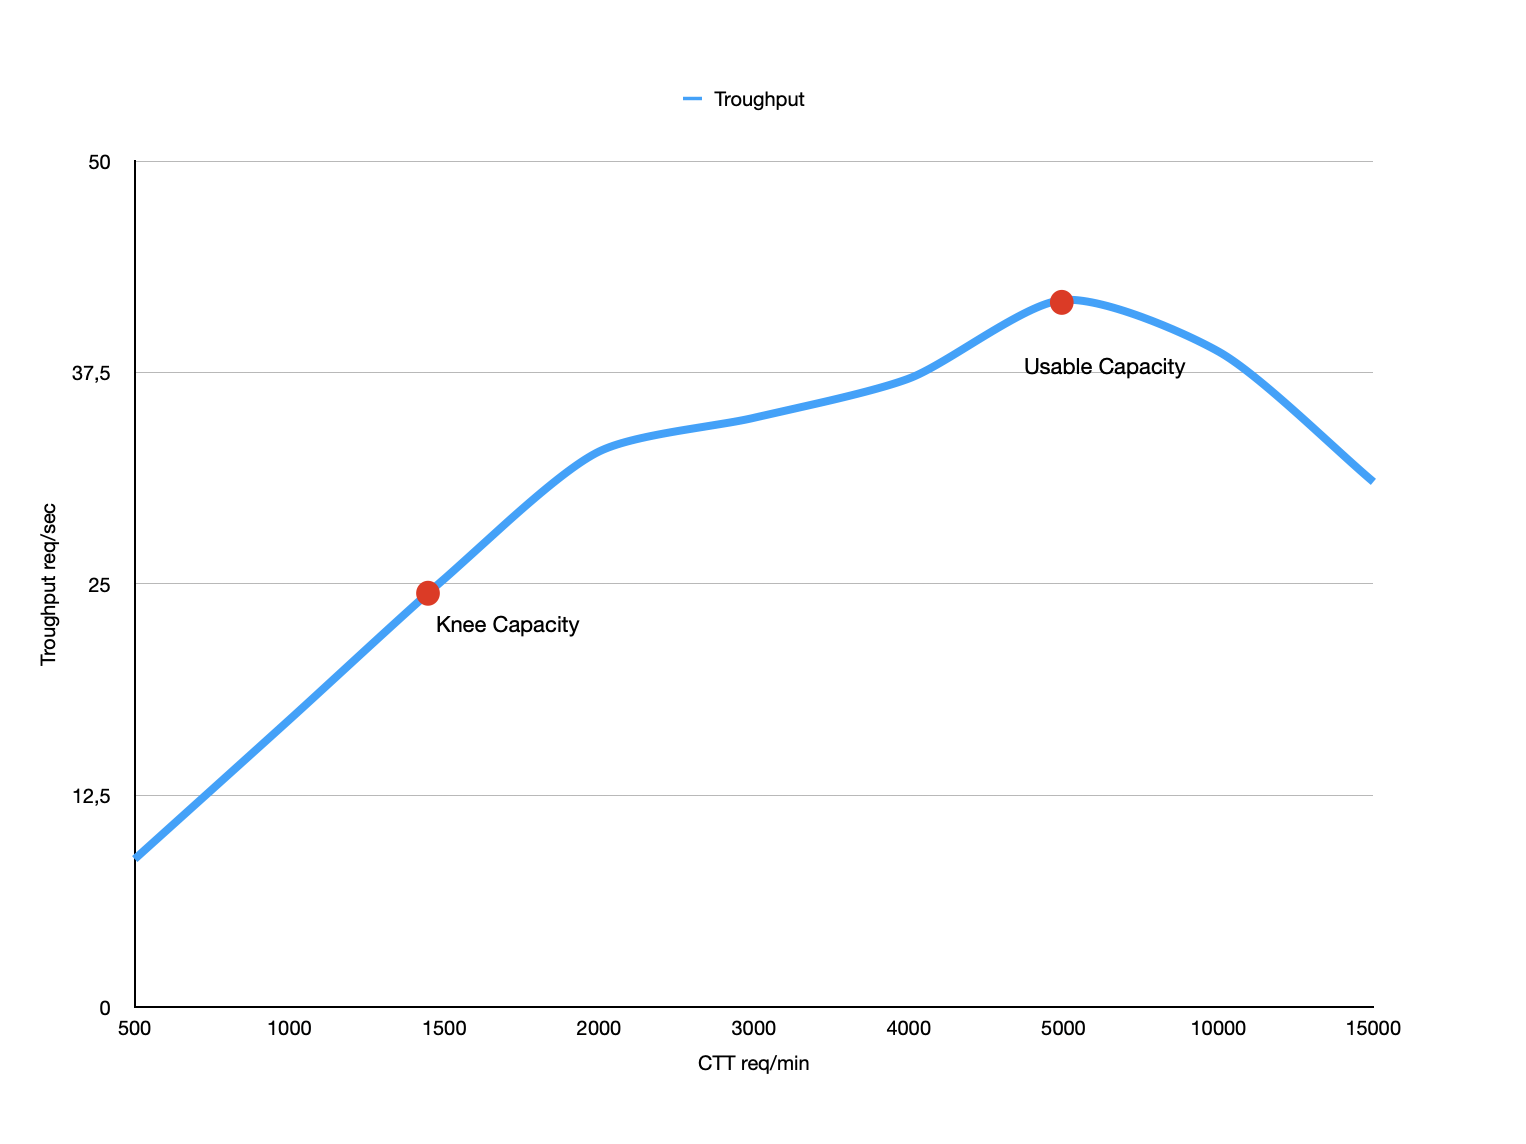
\includegraphics[scale=0.5]{img/chap_1/Througput.png}
    \caption{Throughput}
    \label{fig:thrugh}
\end{figure}
\begin{figure}[H]
    \centering
    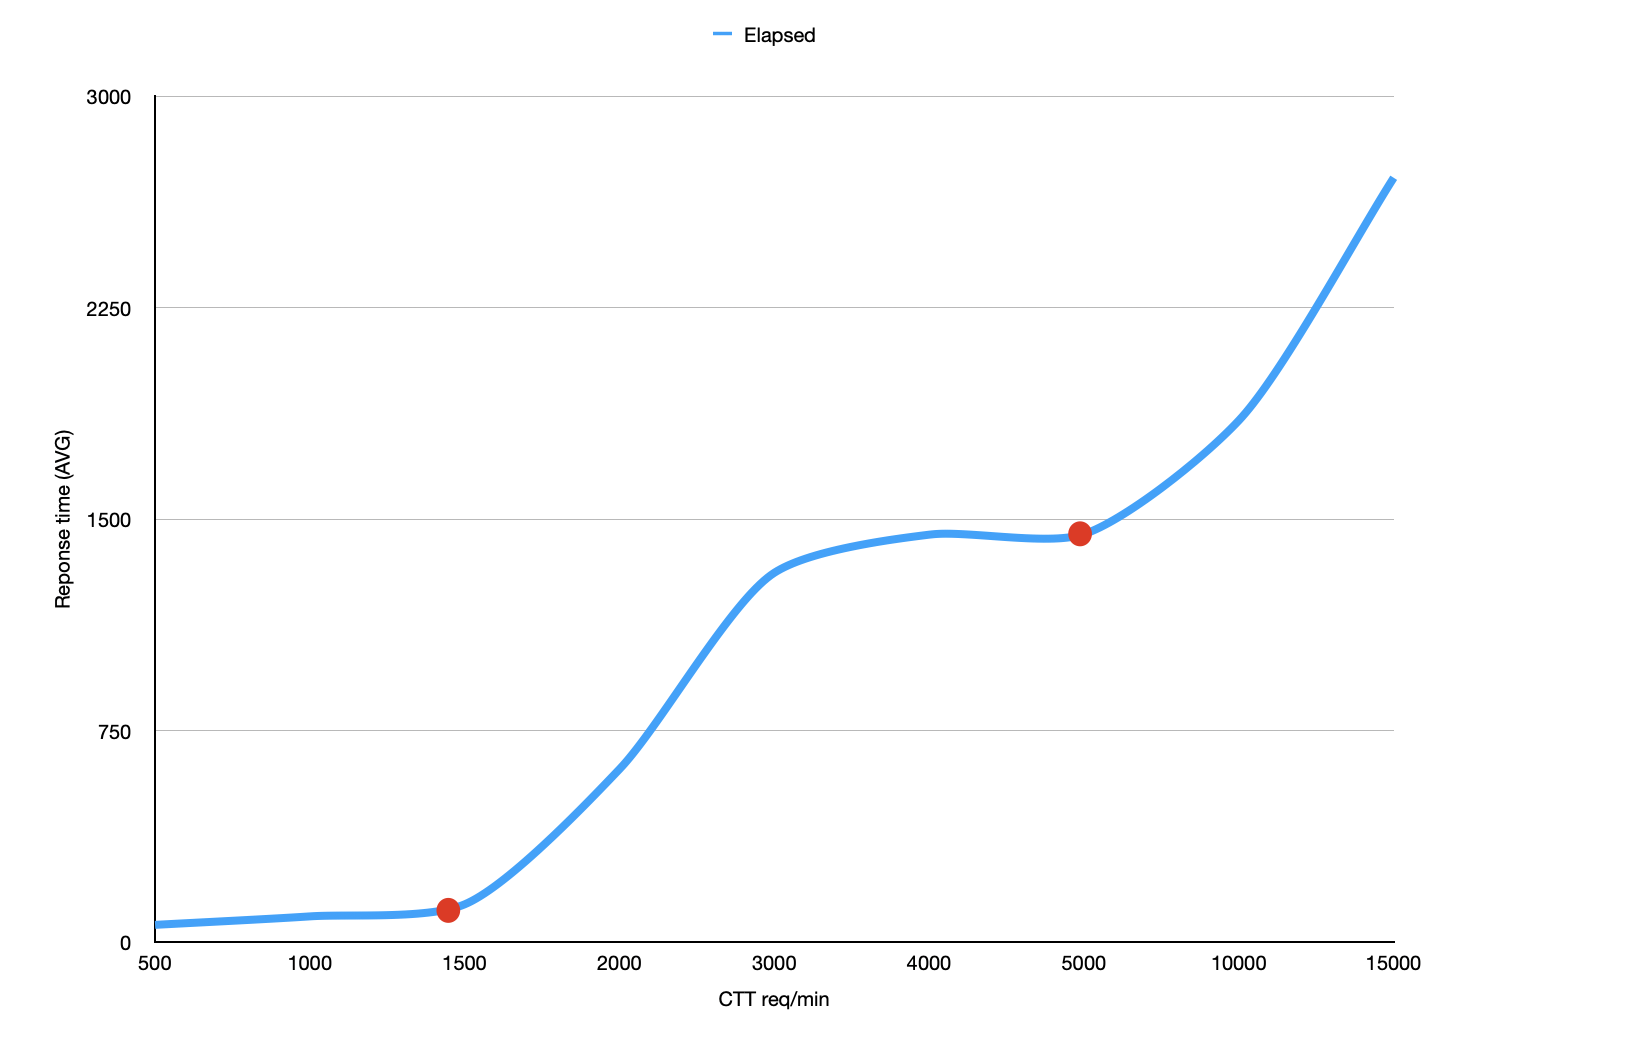
\includegraphics[scale=0.5]{img/chap_1/Response.png}
    \caption{Response}
    \label{fig:response}
\end{figure}
\begin{figure}[H]
    \centering
    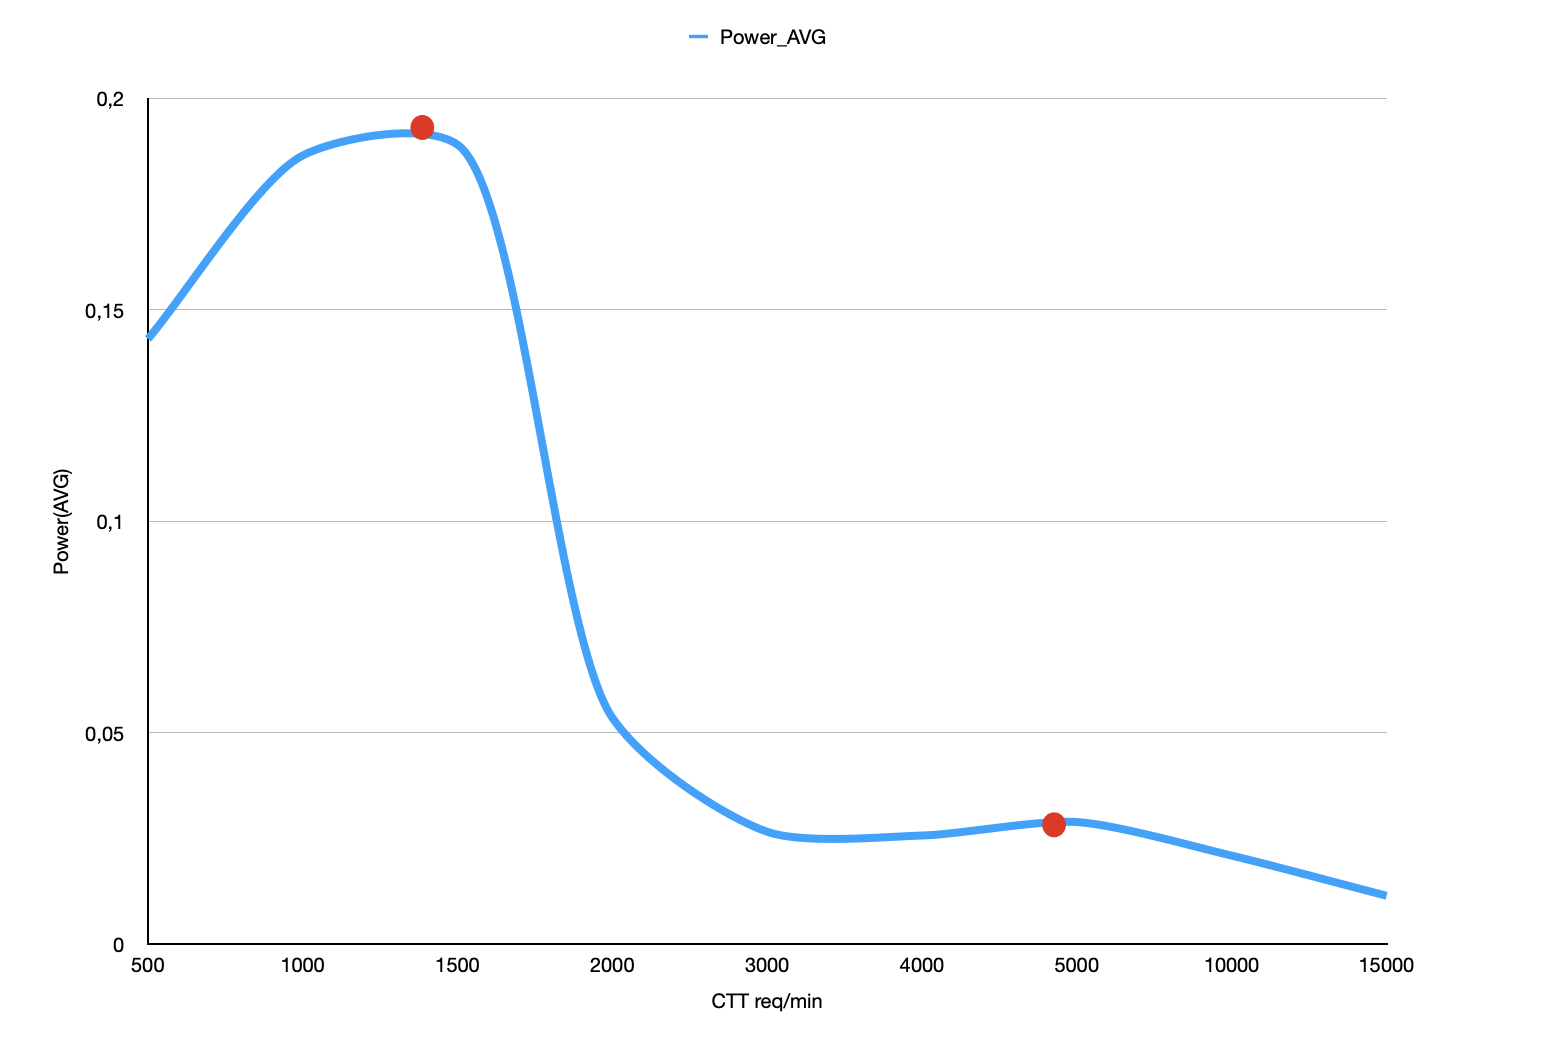
\includegraphics[scale=0.5]{img/chap_1/Power.png}
    \caption{Power}
    \label{fig:power}
\end{figure}
Dai grafici ricavai individuiamo facilmente \textit{Knee Capacity} e \textit{Usable Capacity}:
\begin{itemize}
    \item \textbf{Knee Capacity}: circa 25 req/sec con un carico di 1500 req/min
    \item \textbf{Usable Capacity}: circa 39 req/sec con un carico di 5000 req/min
\end{itemize}
\subsection{Analisi Bottleneck}
Durande la sottomissione delle richieste sono stati analizzati anche i parametri di basso livello del SUT attraverso il tool \textbf{vmstat} con il quale è stato possibile eseguire un analisi per individuare possibile bottleneck del sistema.\\
Ricordiamo che il bottleneck si presenta quando la capacità di esecuzione di un applicazione o computer è limitata da un singolo componente. Il bottleneck è la parte che presenta il mior throughput di tutte le parti. 
Anche in questa fase sono stati calcolati indici come media e coefficiente di variazione per definire se fosse meglio usare la media o la mediana e dai dati raccolti si è ritenuto opportuno usare la media.\\
Dalle analisi risulta che il sistema CPU presenta un bottleneck poichè il parametro \textbf{id}, che secondo la documentazione vmstat rappresenta la percentuale di tempo in idle, è quasi perennemente allo 0\% come dimostrato dal successivo grafico.
\begin{figure}[H]
    \centering
    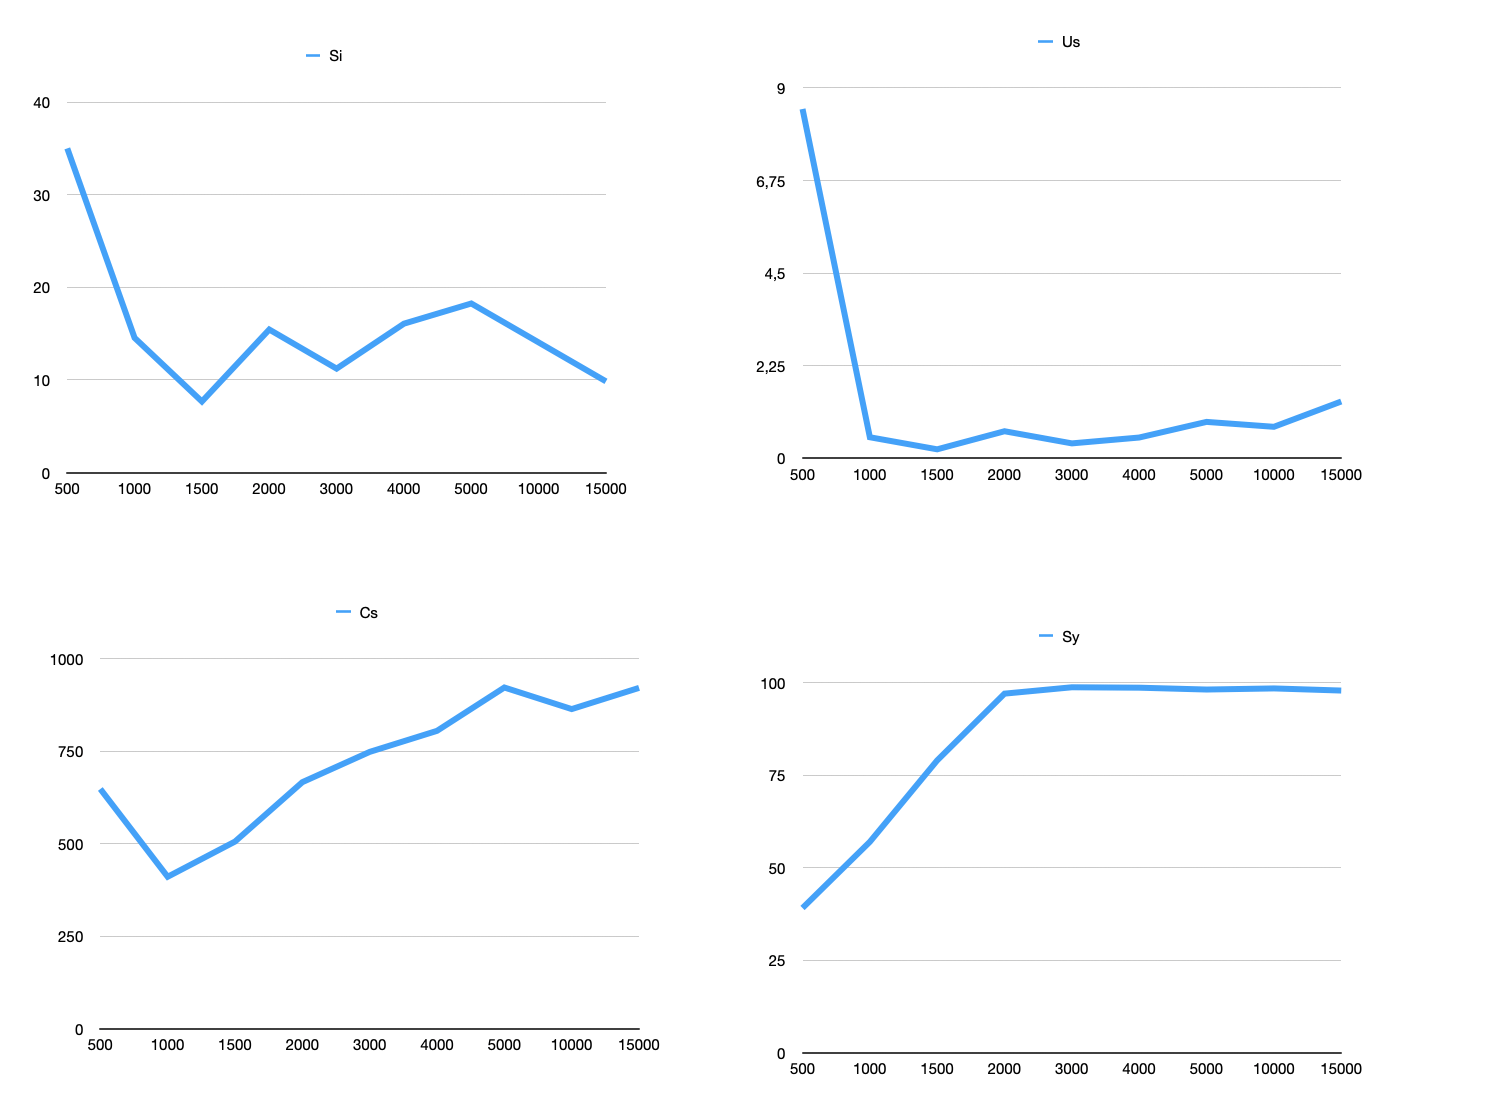
\includegraphics[scale=0.5]{img/chap_1/Bottleneck.png}
    \caption{Parametri CPU vmstat}
    \label{fig:bottleneck}
\end{figure}
\noindent
Per provare la significatività dei risultati si è deciso di effettuare un DoE one factor con 3 ripetizioni in modo da stimare l'errore.\\
Avendo raccolto i dati necessari è stato valutato il modello come si può osservare di seguito.
\begin{figure}[H]
    \centering
    \includegraphics[scale=0.5]{img/chap_1/DoEBottleneck.png}
    \caption{Modello DoE Bottleneck}
    \label{fig:doeBott}
\end{figure}
\noindent
Come si può osservare dalla figura \ref{fig:doeBott} possiamo osservare che SSE = $\frac{1998,886}{11744,525}$ = 17\%.\\
Inoltre si è proceduto ad una analisi di significativià.\\
\begin{figure}[H]
    \centering
    \includegraphics[scale=0.5]{img/chap_1/ResiduiNonNormali.png}
    \includegraphics[scale=0.5]{img/chap_1/ShWiRes.png}
    \caption{Normalita residui}
    \label{fig:normRes}
\end{figure}
\noindent
Come si può notare dalla figura \ref{fig:normRes} i residui non sono normali, dunque bisogna usare un test non parametrico come quello di Wilcoxon che dopo averlo effettuato ha dato il seguente risultato.
\begin{figure}[H]
    \centering
    \includegraphics[scale=0.5]{img/chap_1/WilcoxonBottl.png}
    \caption{Wilcoxon Bottleneck}
    \label{fig:WilcoxBottl}
\end{figure}
\noindent
Come è possibile osservare dal test in figura \ref{fig:WilcoxBottl} abbiamo una significatività statistica e non semplice casualità.
\subsection{Indice di equità}
Tamite Apache Jmeter è stato creato un tesplan con 3 thread-group che richiedono in modo concorrente allo stesso Web Server le 9 risorse disposte.\\
Attraverso i CTT di questi thread group sono stati definiti i seguenti fair throughput:
\begin{itemize}
    \item Thread group 1: 800 req/min
    \item Thread group 2: 300 req/min
    \item Thread group 3: 400 req/min
\end{itemize}
Attraverso il summary report sono stati misurati i seguenti throughput:

\begin{itemize}
    \item Thread group 1: 372 req/min
    \item Thread group 2: 240 req/min
    \item Thread group 3: 252 req/min
\end{itemize}

I throughput normalizzati $x_{i}$ dati dal rapporto tra throughput misurati e fair sono: 
\begin{itemize}
    \item Thread group 1: 0,465
    \item Thread group 2: 0,8
    \item Thread group 3: 0,63
\end{itemize}
Avendo questi elementi possiamo calcolare l'indice di equità: 
\begin{center}
F\_I= $\frac{(\sum^n_{i=1}{x_i})^2}{n\sum^n_{i=1} (x_i)^2}$     
\end{center}
Allora avrò: 
\begin{center}
   F\_I =  $\frac{(0,465+0,8+0,63)^2}{3(0,465^2+0,8^2+0,63^2)} = \frac{3,591}{3,759}$ = 0,955
\end{center}
Si può notare che il server ha un ottimo indice di Fariness, in particolare osserviamo che è molto fair con il Thread group 2 che prevede il CTT più basso mentra è meno fair nei confronti dal primo thread group.
\section{Workload Characterization}
La workload characterization ha come obiettivo quelli di produrre un modello in grado di catturare il comportamento statico e dinamico di un carico reale cui è soggetto il \textit{System Under Test} (SUT) che sia facile da riprodurre, ripetibile e accurato.\\
La workload characterization effettuata ha come soggetto il web-server discusso in tale capitolo ed è stata sviluppata tramite le seguenti fasi:
\begin{itemize}
    \item definizione del SUT 
    \item definizione di un workload di alto livello reale applicabile al sistema.
    \item raccolta di parametri di alto e basso livello.
    \item caratterizzazione del workload di alto livello, di basso livello e generazione di un workload sintetico di alto livello.
    \item validazione del workload sintetico generato tramite il confronto statistico tra i workload di basso livello caratterizzati.
\end{itemize}
Il processo è descritto dalla seguente figura
\begin{figure}[H]
    \centering
    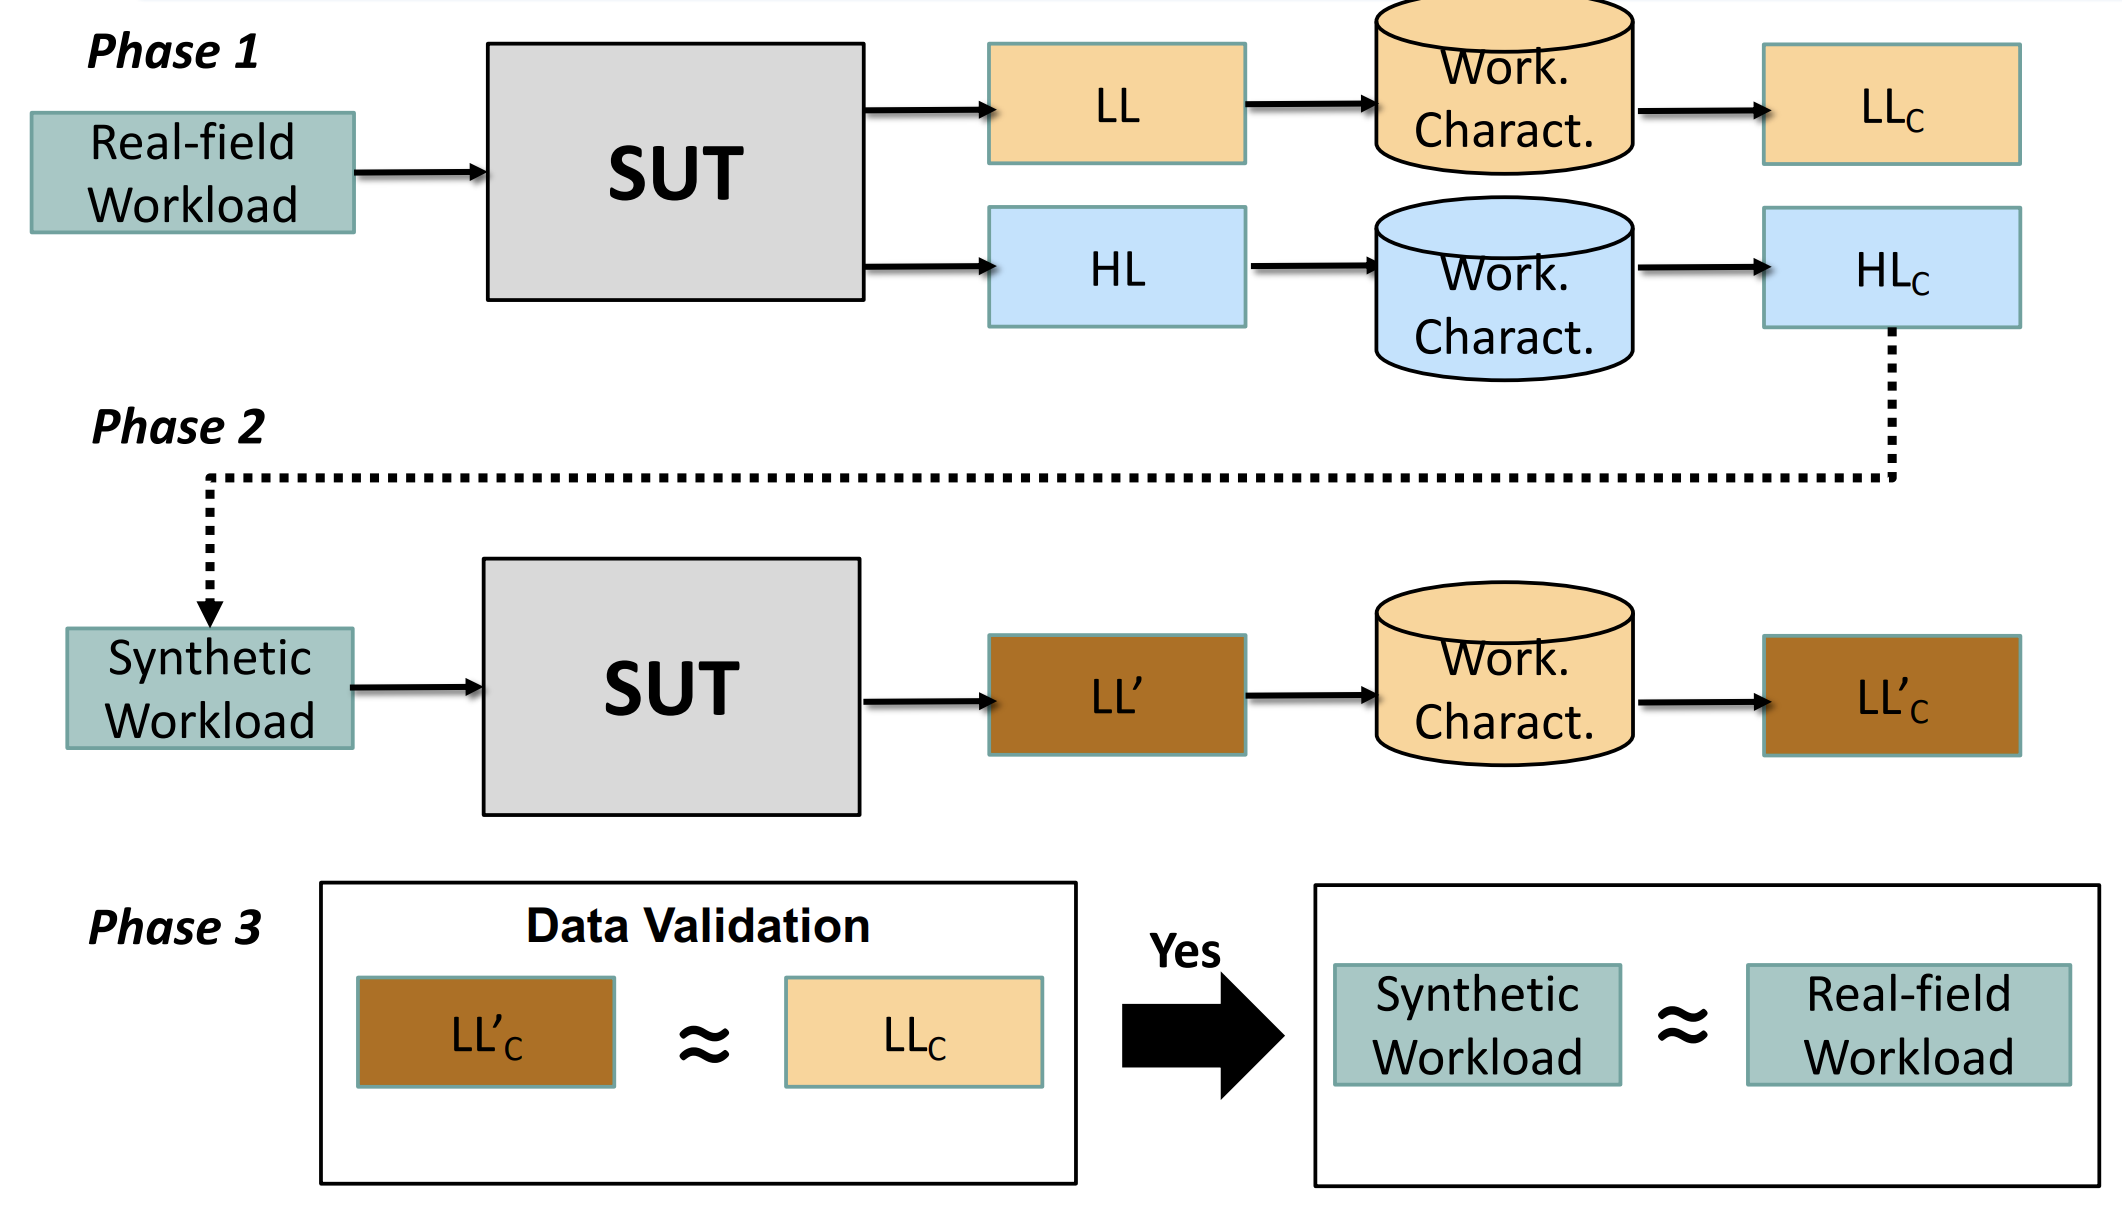
\includegraphics[scale=0.3]{img/chap_1/workLoadCharct.png}
    \caption{Processo di Workload Characterization}
    \label{fig:workLC}
\end{figure}
\subsection{Definizione del SUT}
Il Systema Under Test è un webserver Apache2 in esecuzione su macchina virtuale Oracle Virtual Box.\\
Per eseguire la workload characterization il server è stato provvisto di 40 risorse di dimensioni che variano da 1 KB fino a 20 MB con un passo di 525 KB.\\
Il workload reale di alto livello è stato generato tramite il tool JMeter.\\
Il settaggio del Test plan è il seguente:
\begin{itemize}
    \item 2 Thread Group da 20 Thread ciascuno caratterizzati da un Random Controller e un request rate di 1300 req/min.
    \item ramp up period di 1s.
    \item tempo di esecuzione dei threadgroup pari a 300s l'uno
\end{itemize}
I dati sono stati collezionati tramite un Simple Data Writer e analizzati tramite JMP.\\
Lato server, i parametri sono stati raccolti tramite il tool vmstat e anche loro analizzati con JMP.
\subsection{HL Workload Characterization}
I dati di alto livello raccolti sono stati importati su JMP ed è stata fatta una prima analisi su media e deviazione standard dei prametri.\\
Di seguito riportiamo la taberlla riassuntiva:
\begin{figure}[H]
    \centering
    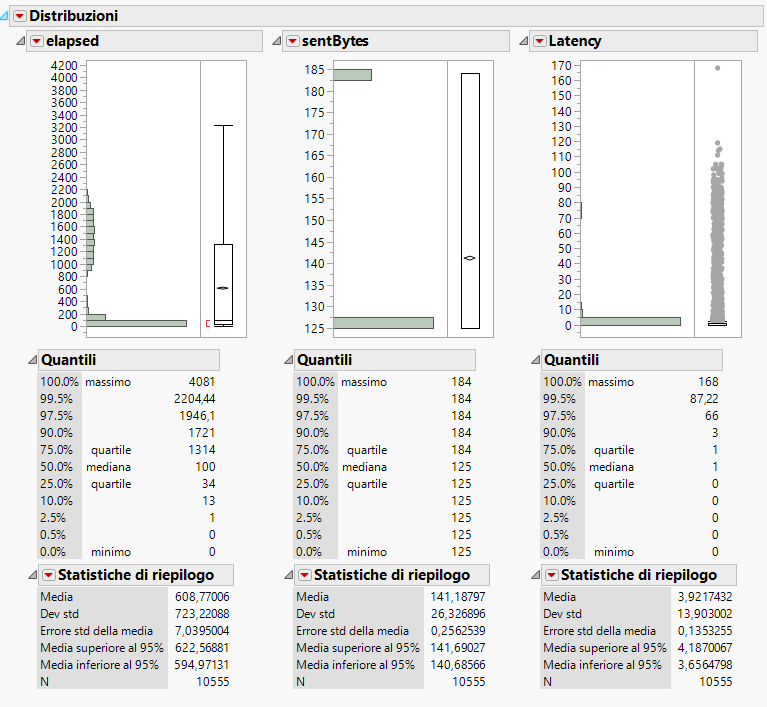
\includegraphics[scale=0.6]{img/chap_1/DistParam_hl.png}
    \caption{Tabella statistiche}
    \label{fig:stats_hl}
\end{figure}
\noindent
Come è possibile osservare dalla tabella \ref{fig:stats_hl} sia \textbf{Sample Count} che \textbf{Error Count} possono essere non considerate come colonne.\\
Una seconda analisi ha interessato le righe.\\
In particolare si è analizzata la presenza o meno di outliers solo per le colonne ritenute utili per l'analisi.\\
\begin{figure}[H]
    \centering
    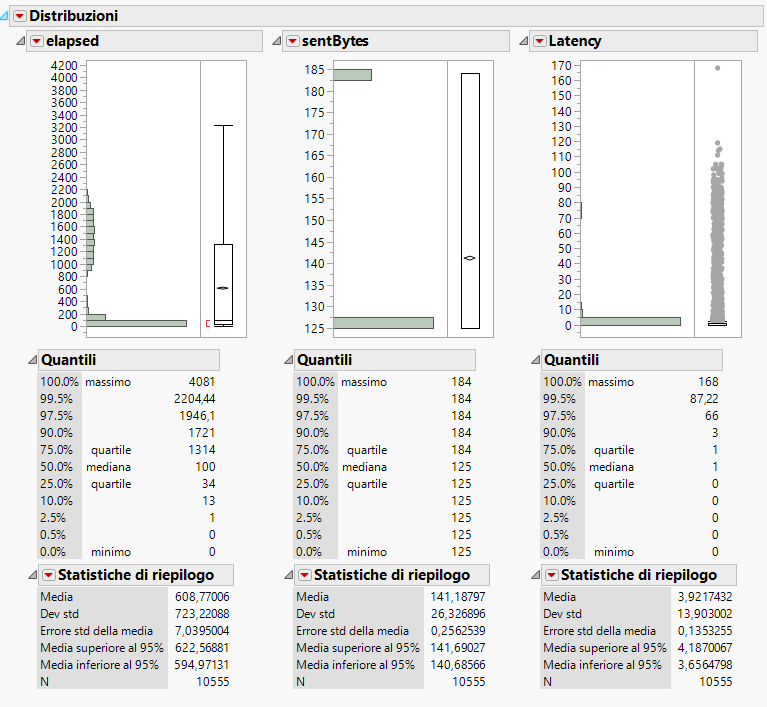
\includegraphics[scale=0.6]{img/chap_1/DistParam_hl.png}
    \caption{Distribuzione dei parametri}
    \label{fig:dist_param}
\end{figure}
\noindent
In tale analisi si è deciso di non filtrare righe poichè non vi sono particolari outliers.\\
Dopodichè è stata eseguita la PCA che riportiamo di seguito:
\begin{figure}[H]
    \centering
    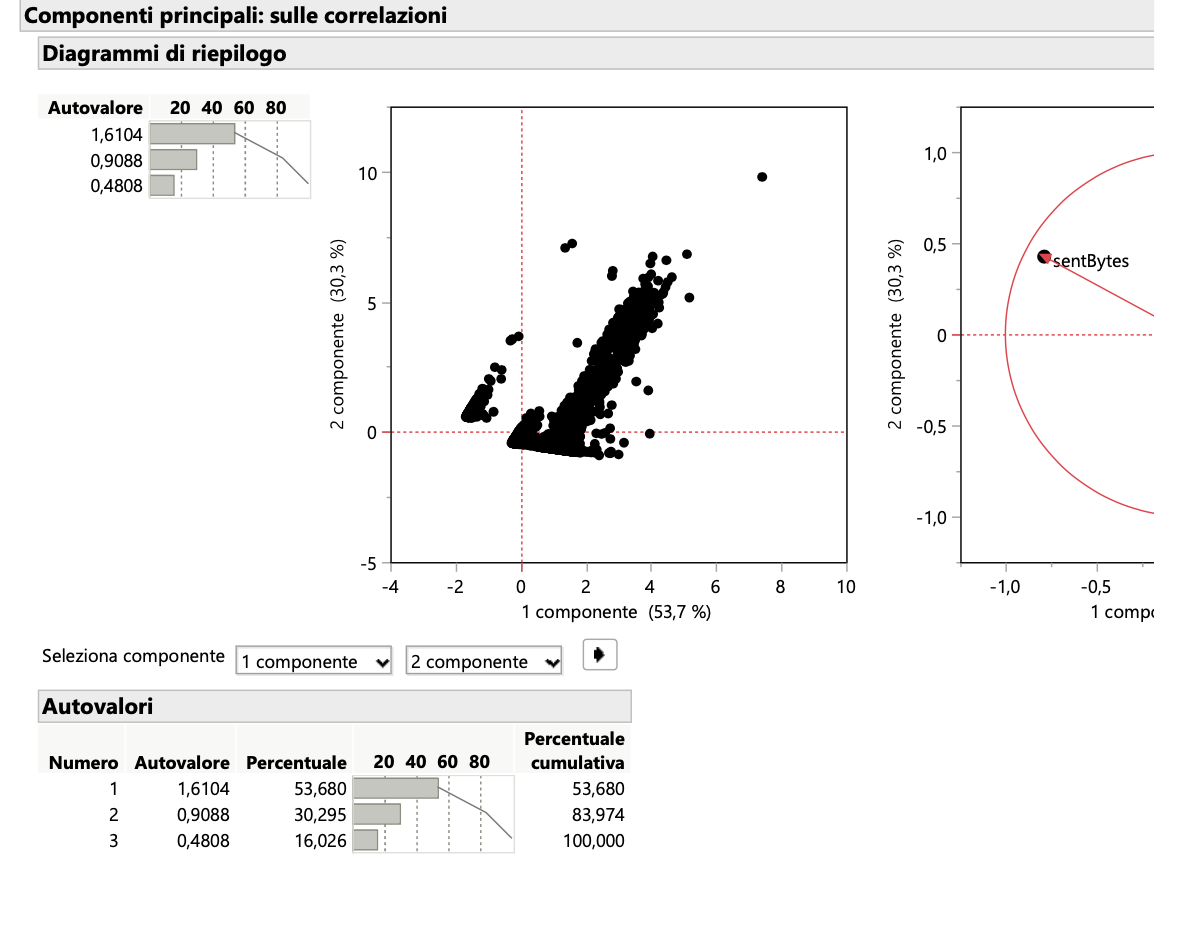
\includegraphics[scale=0.3]{img/chap_1/PCA_HL.png}
    \caption{Clustering HL}
    \label{fig:clust_hl}
\end{figure}
\noindent
Poichè la dimensionalità è molto esigua  si è proceduto a selezionare tutte le componenti principali.\\
Dopo aver effettuato la PCA è stato effettuato il Clustering.\\
Di seguito riportiamo la procedura che JMP ha eseguito 
\begin{figure}[H]
    \centering
    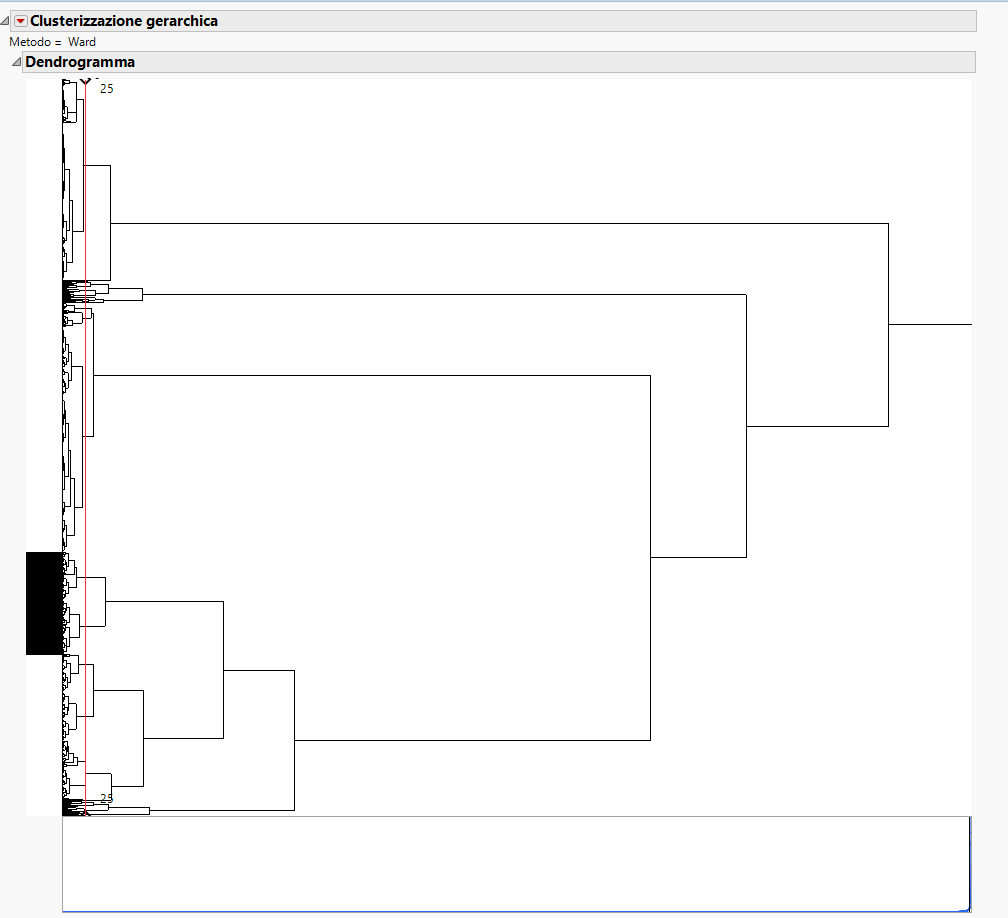
\includegraphics[scale=0.3]{img/chap_1/ClustHL.png}
    \caption{Clustering HL}
    \label{fig:clust_hl}
\end{figure}
\noindent
Osservando la figura in basso al dendogramma abbiamo concluso che il miglior numero di cluster che potevamo contemplare fosse 25 con una perdita dello 0.008\%.\\
\begin{figure}[H]
    \centering
    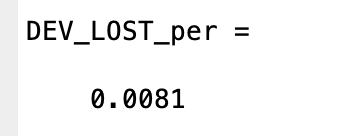
\includegraphics[scale=0.5]{img/chap_1/var_loss_hl.png}
    \caption{Clustering HL}
    \label{fig:clust_hl}
\end{figure}
\noindent
Per scegliere le richieste HTTP si è svolta una analisi di contingenza del parametro label rispetto al cluster attraverso uno script python che seleziona la richiesta più rappresentativa di un determinato cluster (attraverso un approccio frequentista) e la eliminava dal dataset (per evitare che comparisse come richiesta rappresentativa anche di un cluster diverso).\\
Di seguito riportiamo la scelta effettuata dallo script:
\begin{figure}[H]
    \centering
    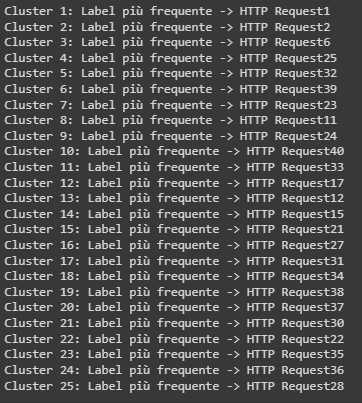
\includegraphics[scale=0.5]{img/chap_1/ChoiceHL.png}
    \caption{Scelta richieste HTTP}
    \label{fig:ch_http_req}
\end{figure}
\noindent
Tale scelta rappresenta anche il Workload sintetico che va riapplicato al SUT.
\subsection{LL Workload Characterization}
La caratterizzazione di basso livello che come obiettivo quello di estrarre punti rappresentativi dei componenti principali con una certa percentuale di varianza spiegata in modo da poterle confrontare con quelle del workload di basso livello ottenuto a seguito dell'applicazione del workload sintetico di alto livello.\\
Anche qui i dati sono stati importati su JMP ed è stata effettuata una analisi su media e deviazione standard.\\
Di seguito riportiamo la tabella riassuntiva:
\begin{figure}[H]
    \centering
    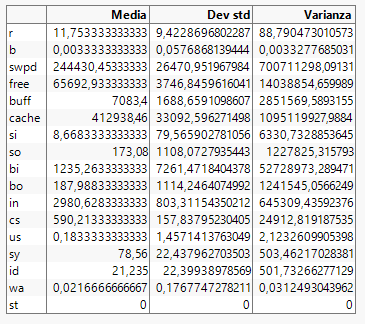
\includegraphics[scale=0.6]{img/chap_1/stats_param_ll1.png}
    \caption{Statistiche LL}
    \label{fig:ll_stats}
\end{figure}
\noindent
Come si può vedere dalla tabella \ref{fig:ll_stats} la colonna \textbf{st} può essere esclusa dalle successive analisi.\\
Anche per questo dataset è stata fatta una analisi sulla distribuzione, ma anche in questo caso non è stato necessario apportare un filtraggio sulle righe del dataset.\\
Si è passati dunque all'analisi multivariata attraverso la PCA che possiamo vedere dalle seguenti figure:
\begin{figure}[H]
    \centering
    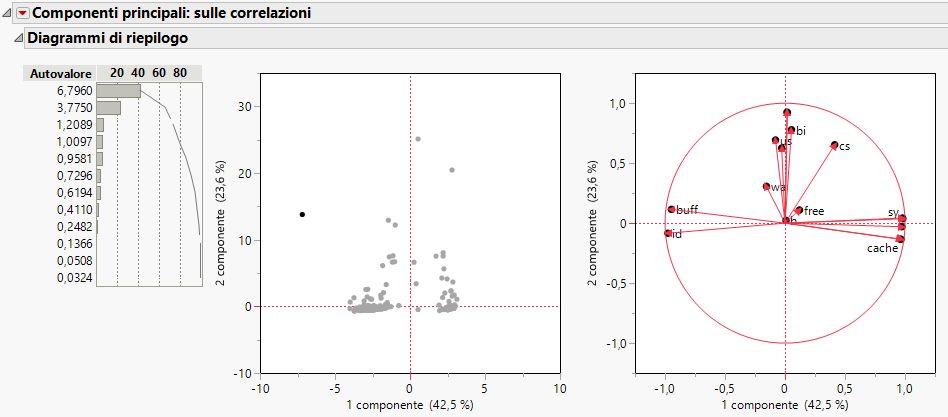
\includegraphics[scale=0.6]{img/chap_1/PCA_1.png}
    \caption{PCA parametri LL}
    \label{fig:pca_ll}
\end{figure}
\noindent
\begin{figure}[H]
    \centering
    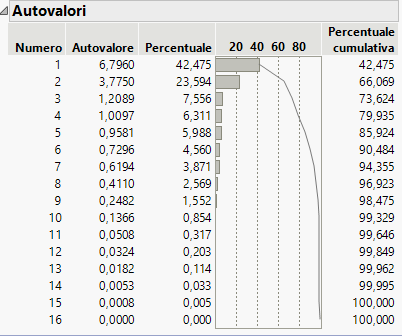
\includegraphics[scale=0.6]{img/chap_1/Autovalori_1.PNG}
    \caption{Autovalori PCA LL}
    \label{fig:autoval_ll}
\end{figure}
\noindent
Dall'analisi multivariata della PCA si è deciso di preservare il 94\% della varianza circa e quindi di selezionare 7 componenti principali.\\
Dopo la procedura di riduzione della dimensionalità delle colonne si è passati al clustering.\\
\begin{figure}[H]
    \centering
    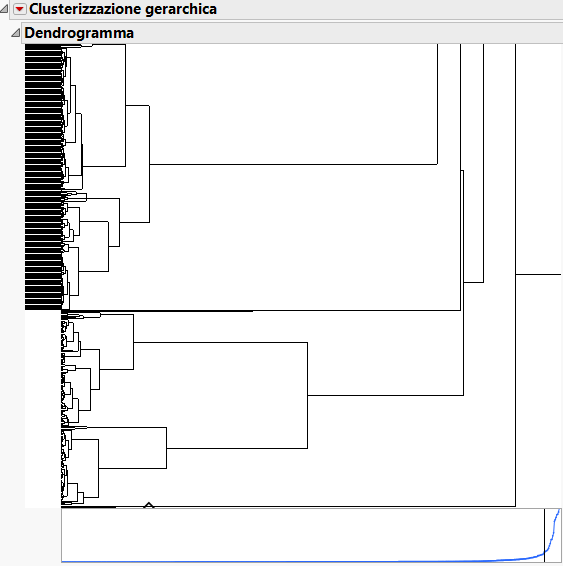
\includegraphics[scale=0.6]{img/chap_1/Clust_1.PNG}
    \caption{Clustering LL}
    \label{fig:clust_ll}
\end{figure}
\noindent
Sempre facendo riferimento al grafico in basso al dendogramma sono stati scelti 20 cluster.\\
Tale scelta ha portato alla perdita di un ulteriore 9\% di varianza.\\
\begin{figure}[H]
    \centering
    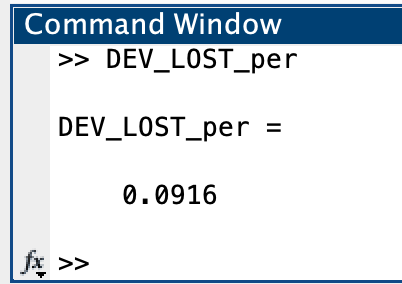
\includegraphics[scale=0.6]{img/chap_1/Varianza_persa_clustering.PNG}
    \caption{Varianza persa LL}
    \label{fig:variance_loss}
\end{figure}
\noindent
Anche in questo caso sono stati scelti tanti parametri quanti sono i cluster, dunque 20.\\
La scelta è stata fatta attraverso uno script Python che ha scelto in maniera randomica i parametri da prendere in considerazione per ogni cluster, producendo il seguente dataset:
\begin{figure}[H]
    \centering
    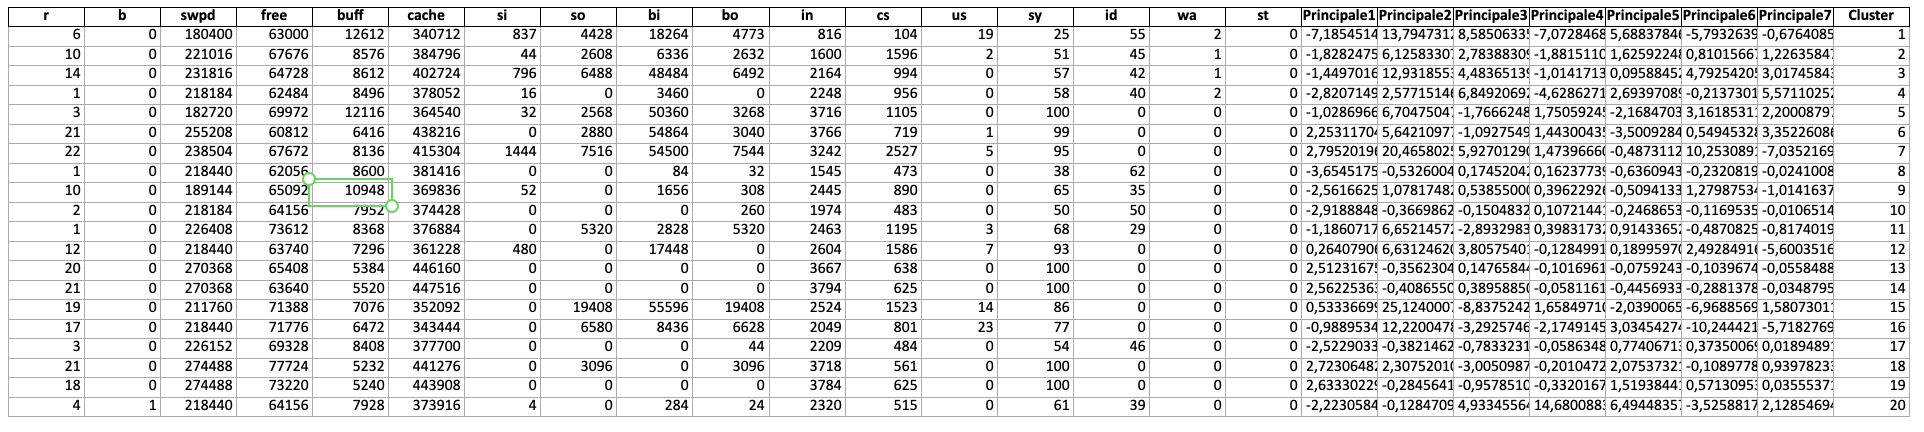
\includegraphics[scale=0.4]{img/chap_1/ll_dataset.png}
    \caption{Dataset LL}
    \label{fig:data_selected_LL}
\end{figure}
\noindent
\subsection{LL' Workload Characterization}
Dopo aver stilato il Workload sintetico, sono state inibite le richieste che non appaiono in quest'ultimo su Jmeter e si è risottoposto il server a questo workload.\\
La sottomissione di questo workload ha prodotto altre statistiche di basso livello di cui si è effettuata l'analisi.\\
In questo caso anche si è effettuata una analisi su media e deviazione standard che però hanno evidenziato ancora che il parametro st non influisca sui dati poichè ha varianza e media nulla.\\
Anche l'analisi sulla distribuzione non ha evidenziato perticolari dati da cancellare.\\
Anche su questi dati è stata effettuata la stessa analisi effettuata per il dataset LL del workload reale, in particolare sono state prese le stesse componenti principali (7) e gli stessi cluster (20) per permettere il confronto statistico tra i due dataset.\\
\subsection{Confronto tra workload}
Per effettuare un confronto statistico dei campioni significativi dei componenti principali , è stata effettuate le seguente considerazione:
\begin{itemize}
    \item \textbf{Verifica di normalità dei campioni}: tale verifica è stata effettuata per capire se è possibile effettuare un test parametrico o non parametrico.\\
    Non abbiamo un numero sufficiente di campioni per assicurarci la normalità secondo il TLC per cui è necessario verificare la normalità dei dati.
\end{itemize}
Di seguito riportiamo i QQ-plot riassuntivi.\\
\begin{figure}[H]
    \centering
    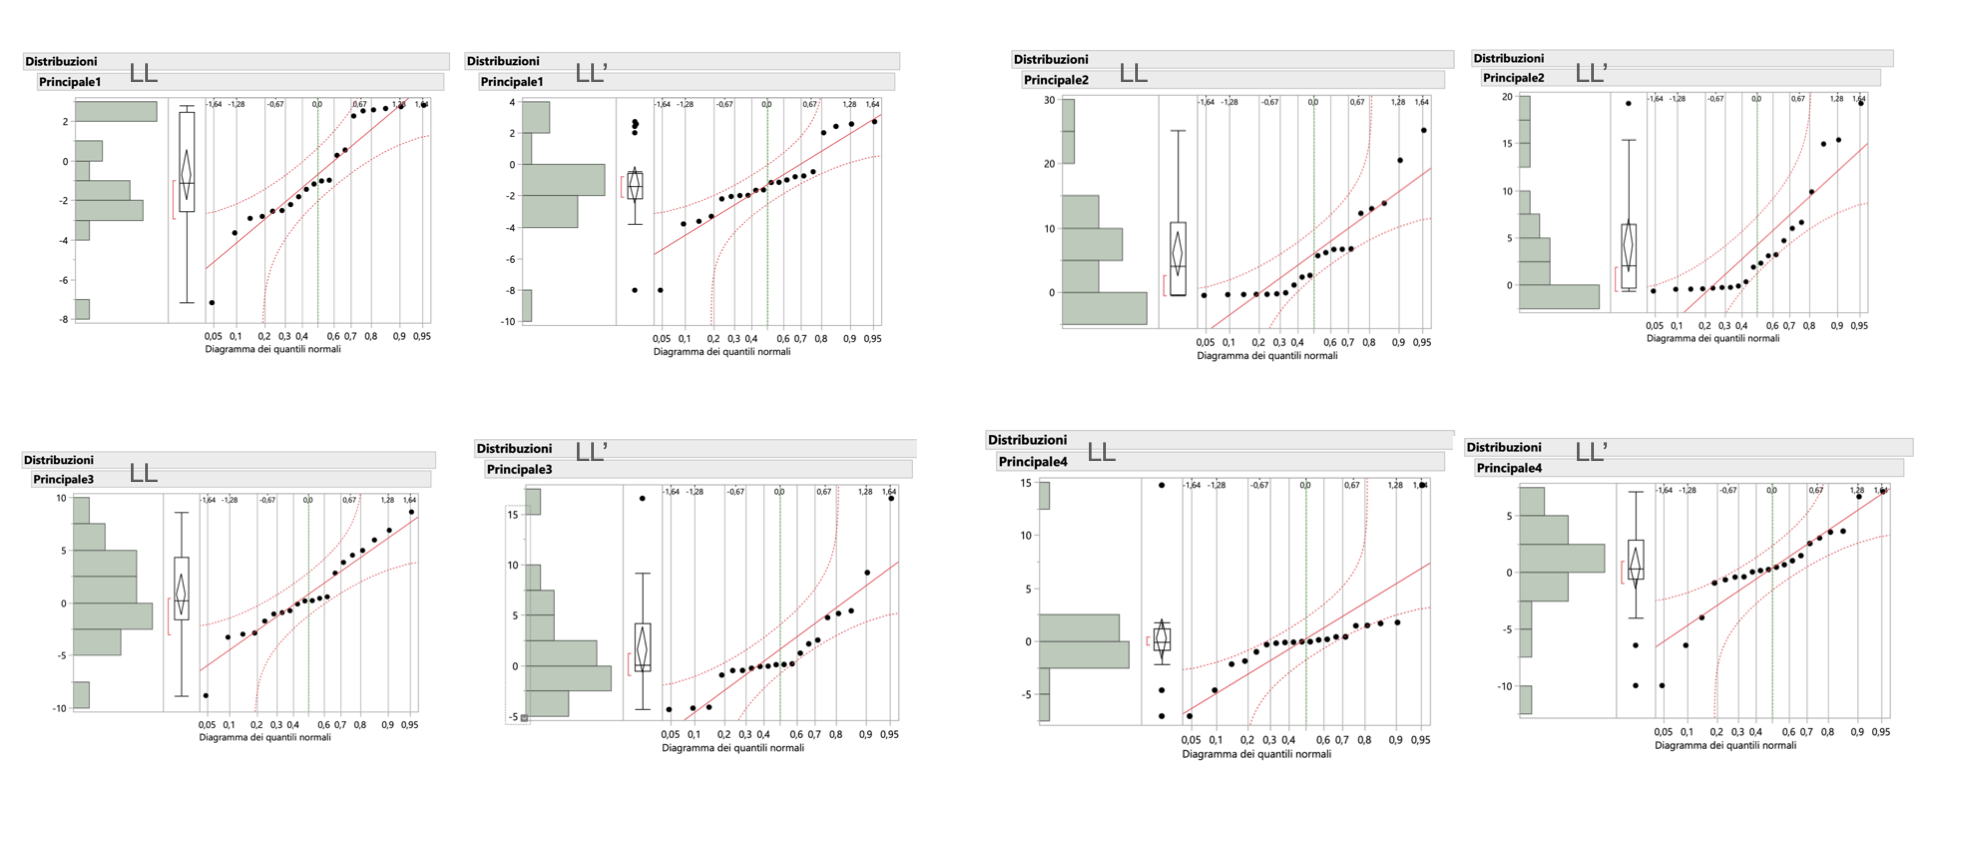
\includegraphics[scale=0.4]{img/chap_1/qq_plots1.png}
    \caption{QQ plot dati LL e LL'}
    \label{fig:qq_plot_ll1}
\end{figure}
\noindent
\begin{figure}[H]
    \centering
    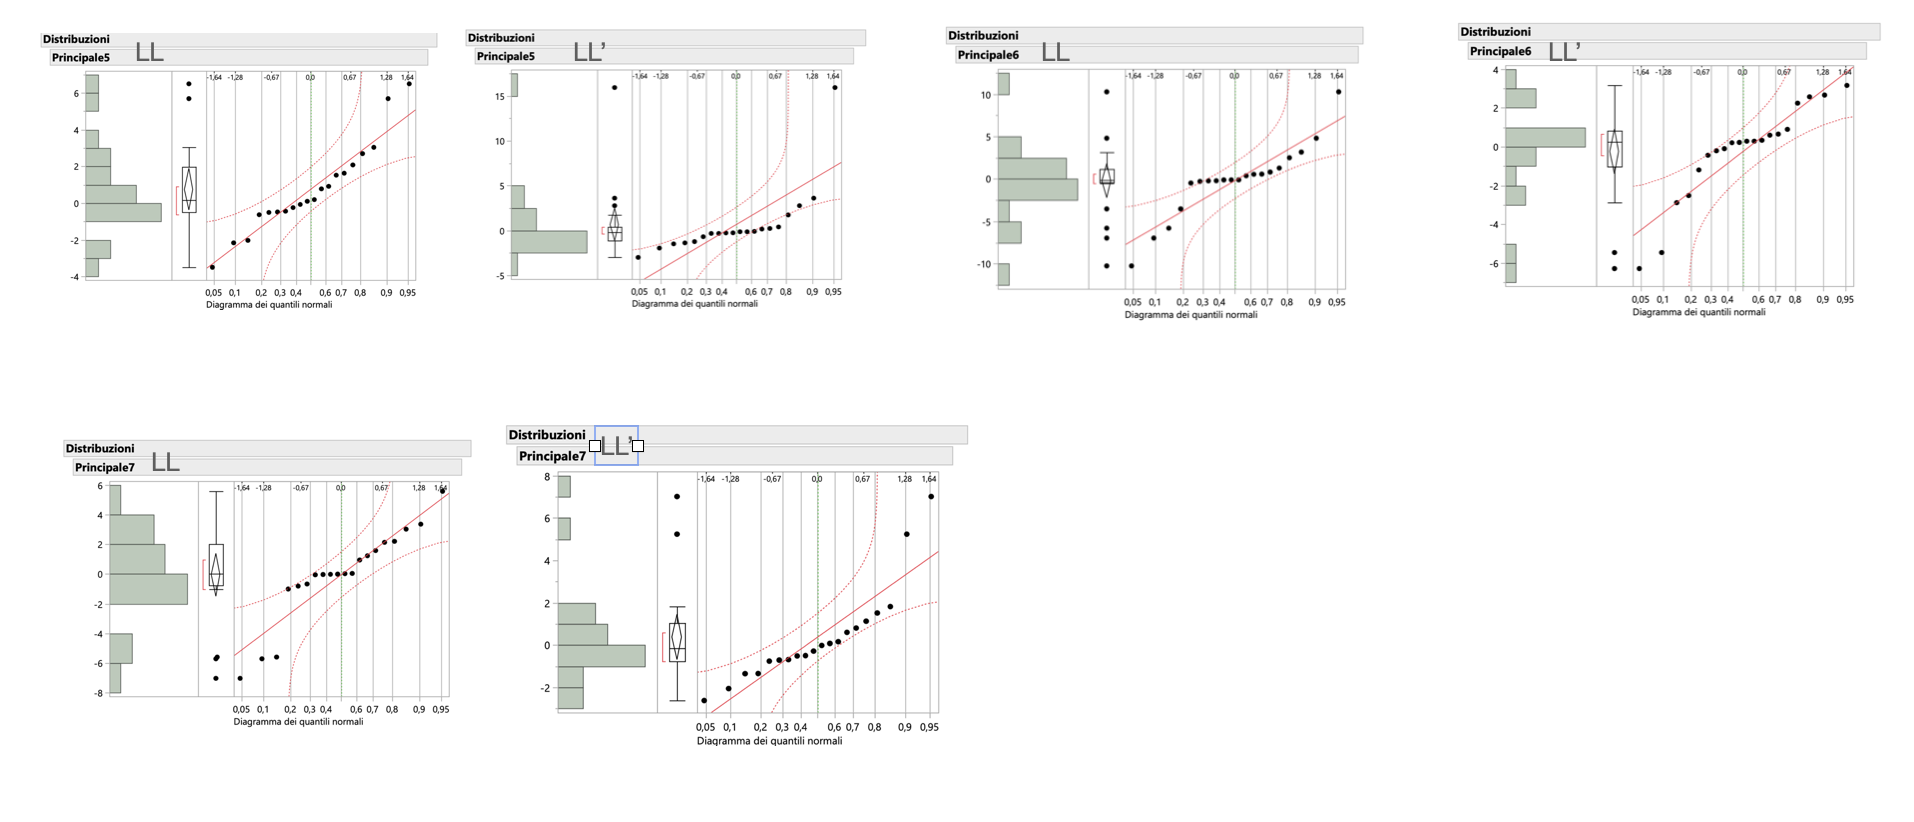
\includegraphics[scale=0.4]{img/chap_1/qq_plots2.png}
    \caption{QQ plot dati LL e LL'}
    \label{fig:qq_plot_ll2}
\end{figure}
\noindent
Dai qq-plots si è deciso di trattare come distribuzioni normali e quindi con test parametrici le componenti principali \textbf{1} e \textbf{7} mentre tutte le altre verranno trattate con test non parametrici.\\
Per queste ultime si è usato il test di Wilcoxon (ranksum su Matlab) di cui riportiamo una tabella con risultato del test e valore del p-value.
\begin{table}[htbp]
    \centering
    \label{tab:esempio}
    \begin{tabular}{|c|c|c|c|} % specifica il numero e l'allineamento delle colonne (c = centrato, l = sinistra, r = destra)
        \hline
        Componente & p-value & Risultato test \\ % separa le celle con '&', e termina ogni riga con '\\'
        \hline
        2 & 0.4570 & 0 \\
        3 & 0.8181 & 0 \\
        4 & 0.3648 & 0\\
        5 & 0.4249 & 0\\
        6 & 0.8817 & 0\\
        \hline
    \end{tabular}
\end{table}
\\
Come Si può vedere la tabella per le componenti principali evidenzate non vi è differenza statistica poichè il test non riesce a rigettare l'ipotesi nulla.\\
Per le componenti 1 e 7 si è proceduto all'uso del T-Test aggregato parametrico, data la normalità dei campioni, che ha dato i seguenti risultati 
\begin{figure}[H]
    \centering
    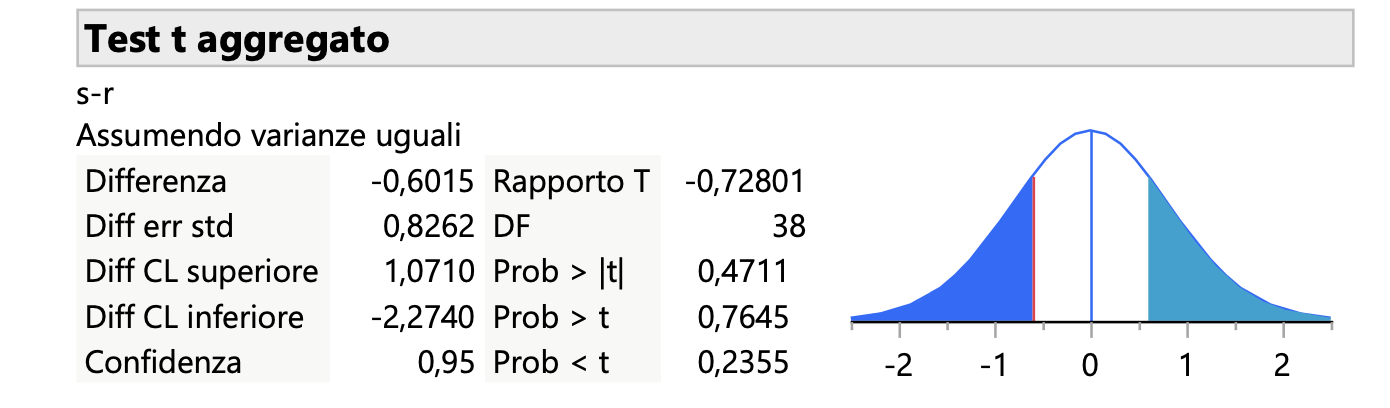
\includegraphics[scale=0.4]{img/chap_1/t_test1.png}
    \caption{T-test componente 1}
    \label{fig:t_test1}
\end{figure}
\noindent
\begin{figure}[H]
    \centering
    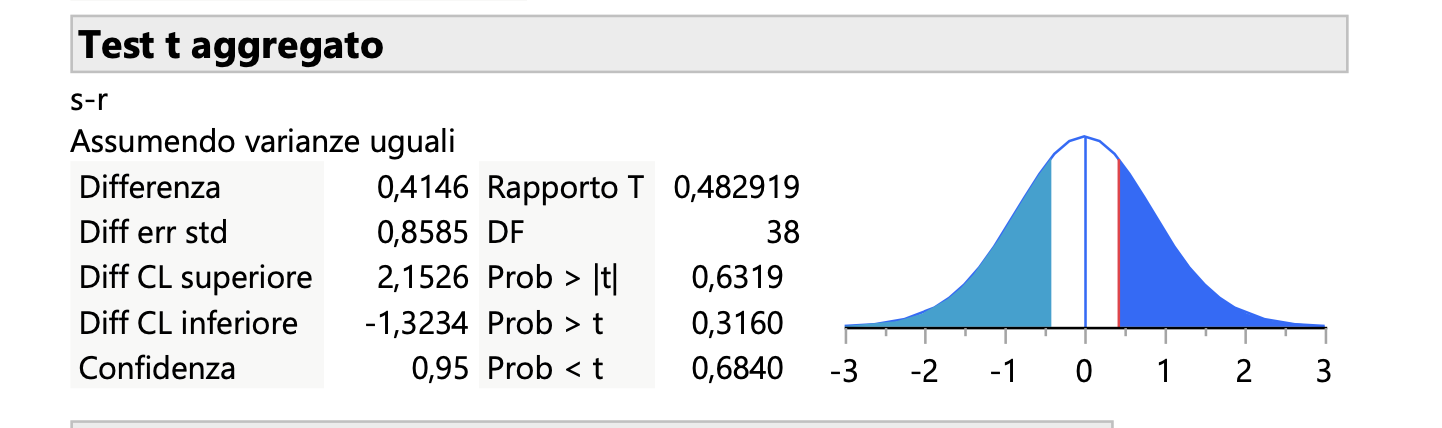
\includegraphics[scale=0.4]{img/chap_1/t_test2.png}
    \caption{T-test componente 7}
    \label{fig:t_test2}
\end{figure}
\noindent
Entrambe i test non rigettano l'ipotesi nulla e quindi con il 95\% di confidenza possiamo affermare che non vi sia differenza statistica per le popolazioni da cui sono stati estratti i campioni.
\section{DoE}
In questo paragrafo descriveremo il processo di creazione di un piano sperimentale detto \textbf{Design of experiment}.\\
Tale processo permette di determinare quali sono i fattori che più influiscono su una particolare metrica di performance misurata sul SUT.\\
Le variabili che influenzano l'uscita sono detti fattori e ad ogni fattore sono associati dei livelli, ovvero valori che il fattore può assumere.\\
Il SUT in esame è sempre il webserver di questo capitolo e le richieste al sistema saranno effettuate sempre tramite apache JMeter.\\
Per il piano attuato abbiamo:
\begin{itemize}
    \item \textbf{Intensità}: indica il carico imposto al sistema e ha 3 livelli low( 25\% della usable capacity), medium(50\% della usable capacity) e high (75\% della usable capacity).
    Dato che la usable capacity è stata individuata a 5000 req/min avrò la low a 1250 req/min, medium 2500 req/min e la high a 3750 req/min.

    \item \textbf{Page size}: dimensione della pagina richiesta al webserver. Il fattore è caratterizzato da 4 livelli small (1KB - 550 KB), medium ( 551KB - 1 MB), large (1MB - 10MB)  
\end{itemize}
Come variabile di risposta si è scelto il response time definito come il tempo che il server impiega a servire una richiesta indirizzata ad una certa risorsa con una determinata intensità e quindi è selezionato come la media degli elapsed.\\
Il numero di ripetizioni fissato per il piano è 5 ripetizioni per definire l'errrore di stima degli effetti dei fattori.\\
Il piano sperimentale è di tipo \textbf{full factorial} e questo ci porta ad eseguire $3^2 \cdot 5 = 45$ esperimenti.\\
Di seguito riportiamo gli esperimenti:
\begin{figure}[H]
    \centering
    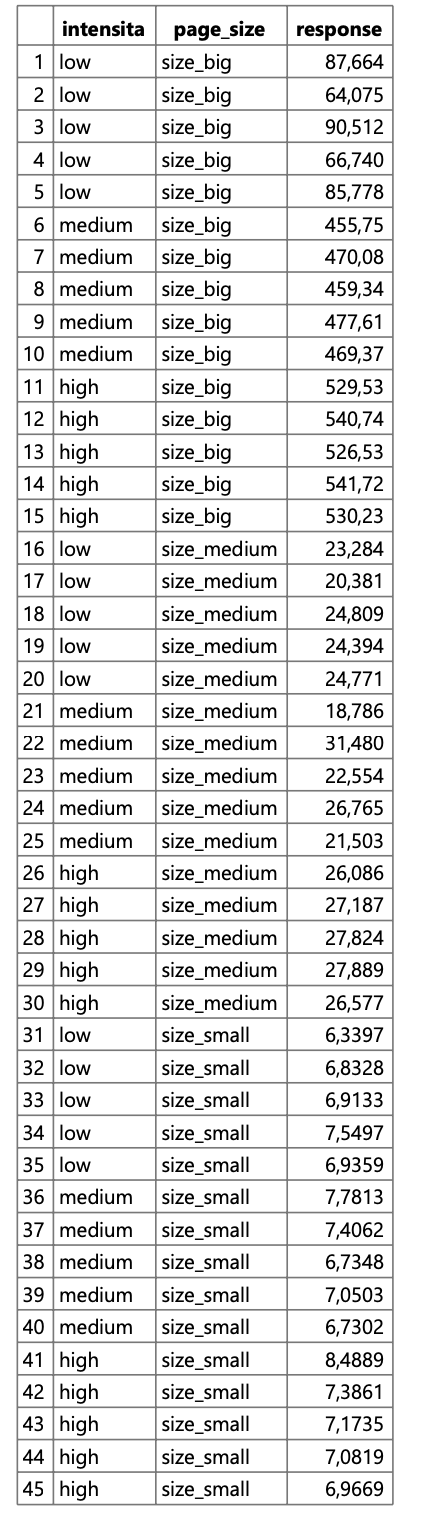
\includegraphics[scale=0.4]{img/chap_1/exp_doe.png}
    \caption{Esperimenti}
    \label{fig:exp_doe}
\end{figure}
\noindent
Una volta effettuati gli esperimenti abbiamo definito, tramite JMP, l'importanza di ogni fattore.\\
Avremo il seguente risultato:
\begin{figure}[H]
    \centering
    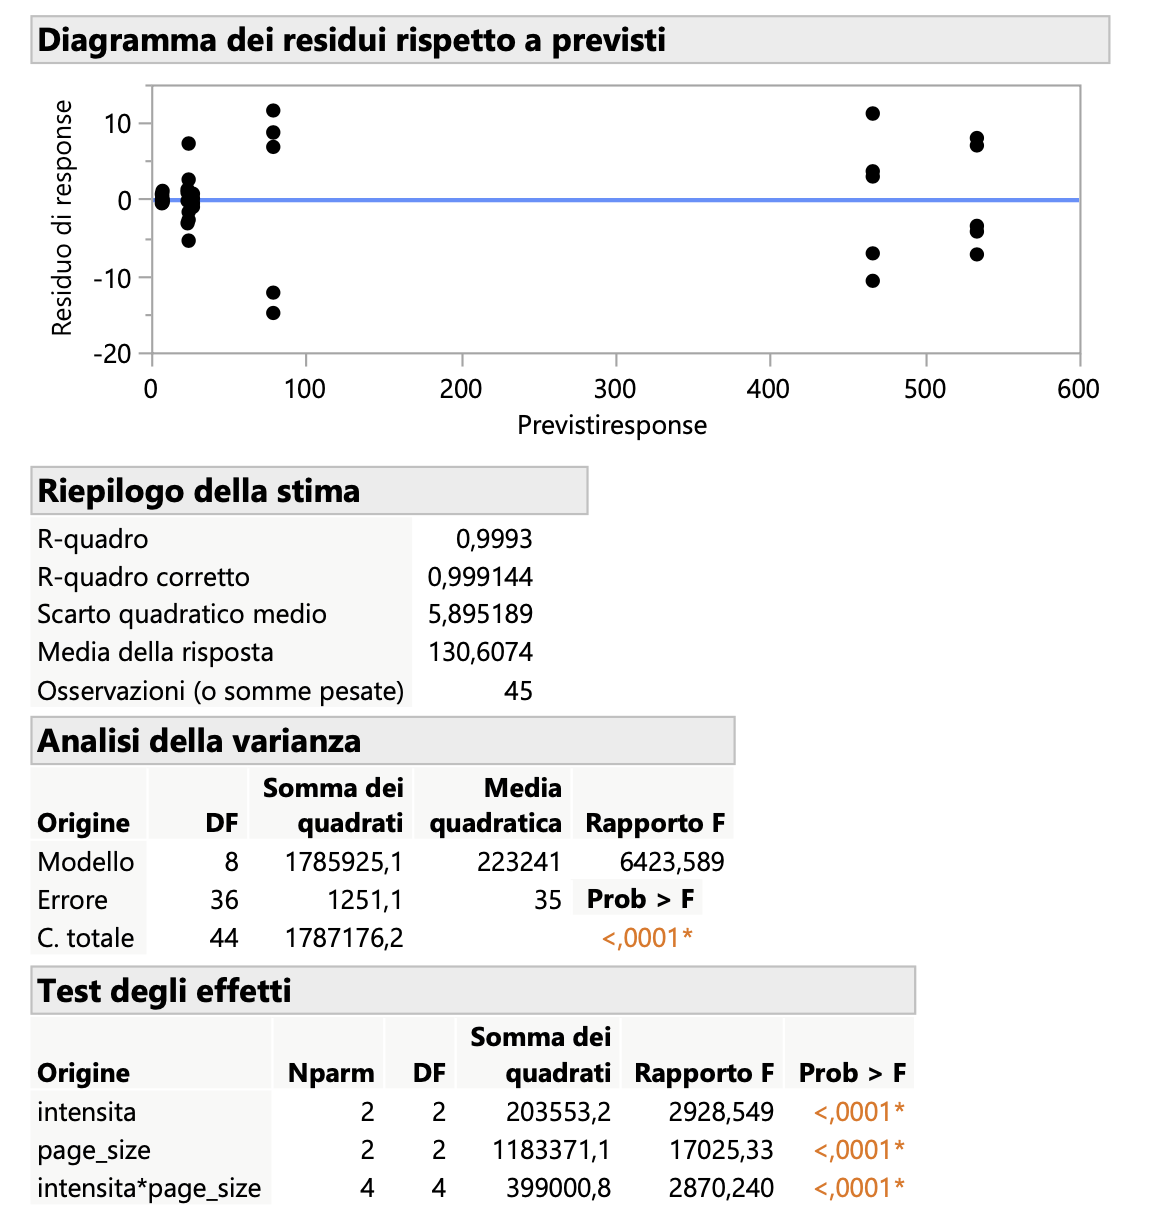
\includegraphics[scale=0.4]{img/chap_1/var_alloc.png}
    \caption{Allocazione della varianza}
    \label{fig:var_alloc}
\end{figure}
\noindent
Come si può osservare dall'analisi della varianza una grande parte della varianza è spiegata dal modello, inoltre una grande parte di quest'ultima è allocata al fattore \textit{page\_size}.\\
Possiamo definire l'importanza facendo il rapporto tra varianza allocata al fattore e quella totale.\\
Avremo dunque:
\begin{center}
    
    $\frac{SSE}{SST} = \frac{1251}{1787176,2} = 0,0006\% $\\
    $\frac{SS_{intensity}}{SST} = \frac{203553,2}{1787176,2} = 11\%$ \\
    $\frac{SS_{pageSize}}{SST} = \frac{1183371,1}{1787176,2}=66\%$ \\
    $\frac{SS_{interaction}}{SST} = \frac{399000,8}{1787176,2}=22\% $
    
\end{center}
Da questa analisi possiamo ottenere una descrizione sull'importanza dei fattori nella risposta.\\
Il fattore fondamentale come si può vedere è il \textit{page\_size} portando con se il 66\% della varianza complessiva.\\
Inoltre è importante anche l'interazione che porta con se il 22\% della varianza.\\
L'errore come si può facimente osservare risulta marginale e associato dunque ad una percentuale di varianza molto piccola.\\
Fatta una analisi sull'importanza possiamo passare ad una analisi riguardo la significativià.\\
In particolare per lo studio è stata utilizzata l'ANOVA (Analysis of Variance).\\
Ricordiamo che la \textbf{significatività} ci dice che quello che abbiamo osservato non è frutto dell'aleatorietà.\\
Per determinare quale tipo di ANOVA si è condotta una analisi sulla distribuzione dei residui, ovvero attraverso un QQ-plot si è verificato che questi residui siano normali.\\
\begin{figure}[H]
    \centering
    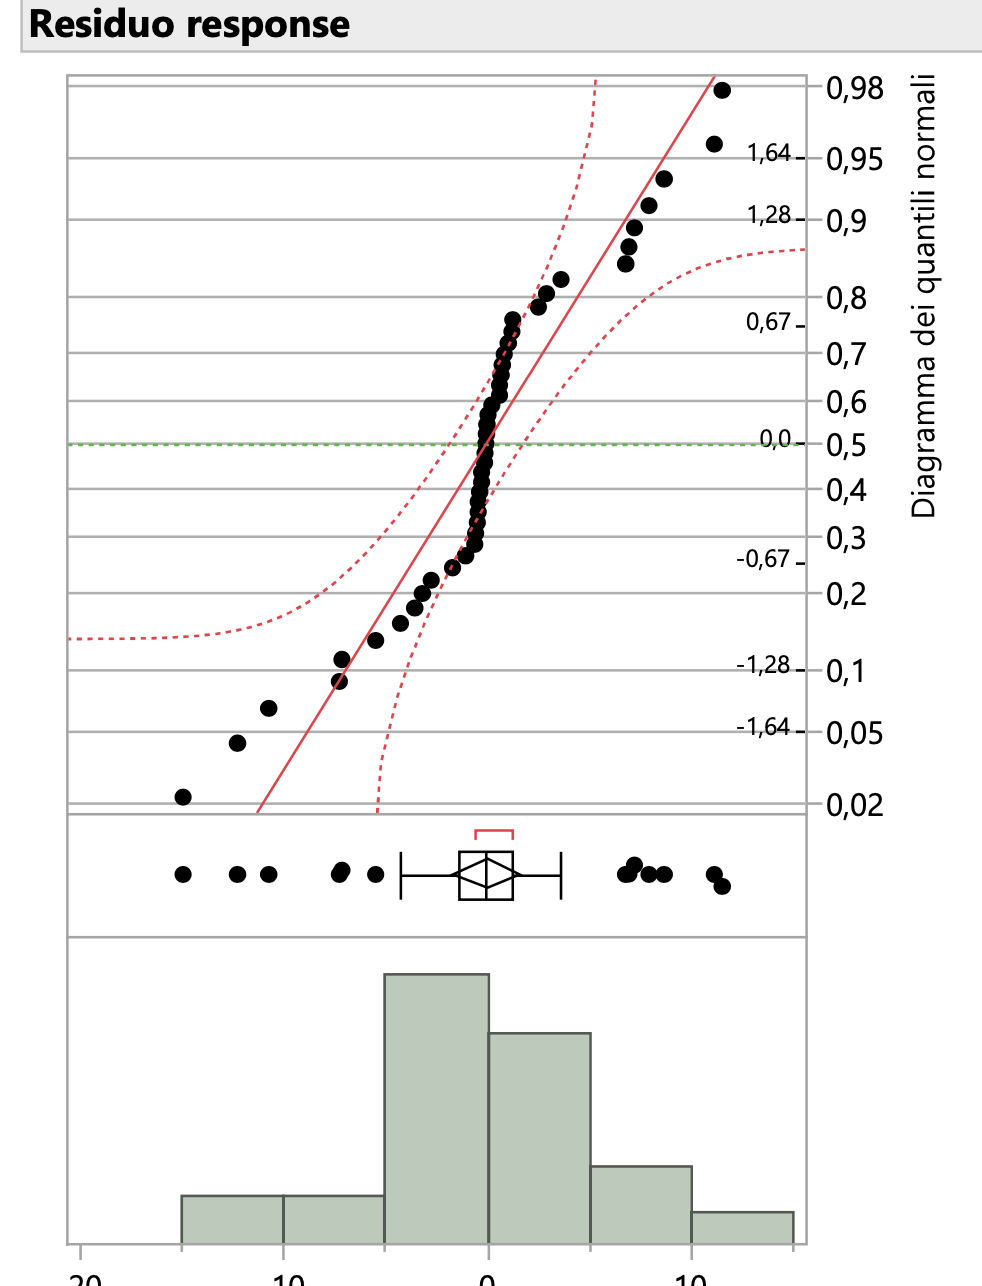
\includegraphics[scale=0.4]{img/chap_1/res_norm.png}
    \caption{qq-plot residui}
    \label{fig:qq_res_plot}
\end{figure}
\begin{figure}[H]
    \centering
    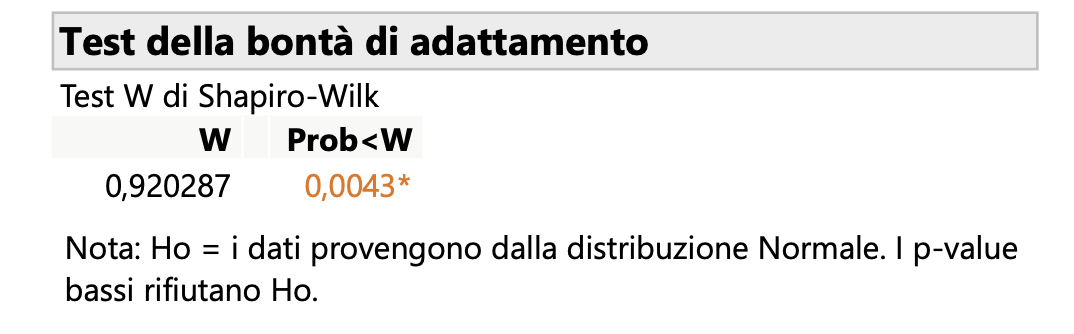
\includegraphics[scale=0.4]{img/chap_1/shwk.png}
    \caption{Test di Shapiro-Wilk}
    \label{fig:shapWilk}
\end{figure}
\noindent
Come si può osservare dalla fidura \ref{fig:qq_res_plot} i residui non sono normali, ipotesi confermata anche da test di Shapiro-Wilk della figura \ref{fig:shapWilk}.\\
Data la non normalità dei campioni si deve procedere per test non parametrici come quello di Kruskal-Wallis, di seguito riportiamo i risultati.\\
\begin{figure}[H]
    \centering
    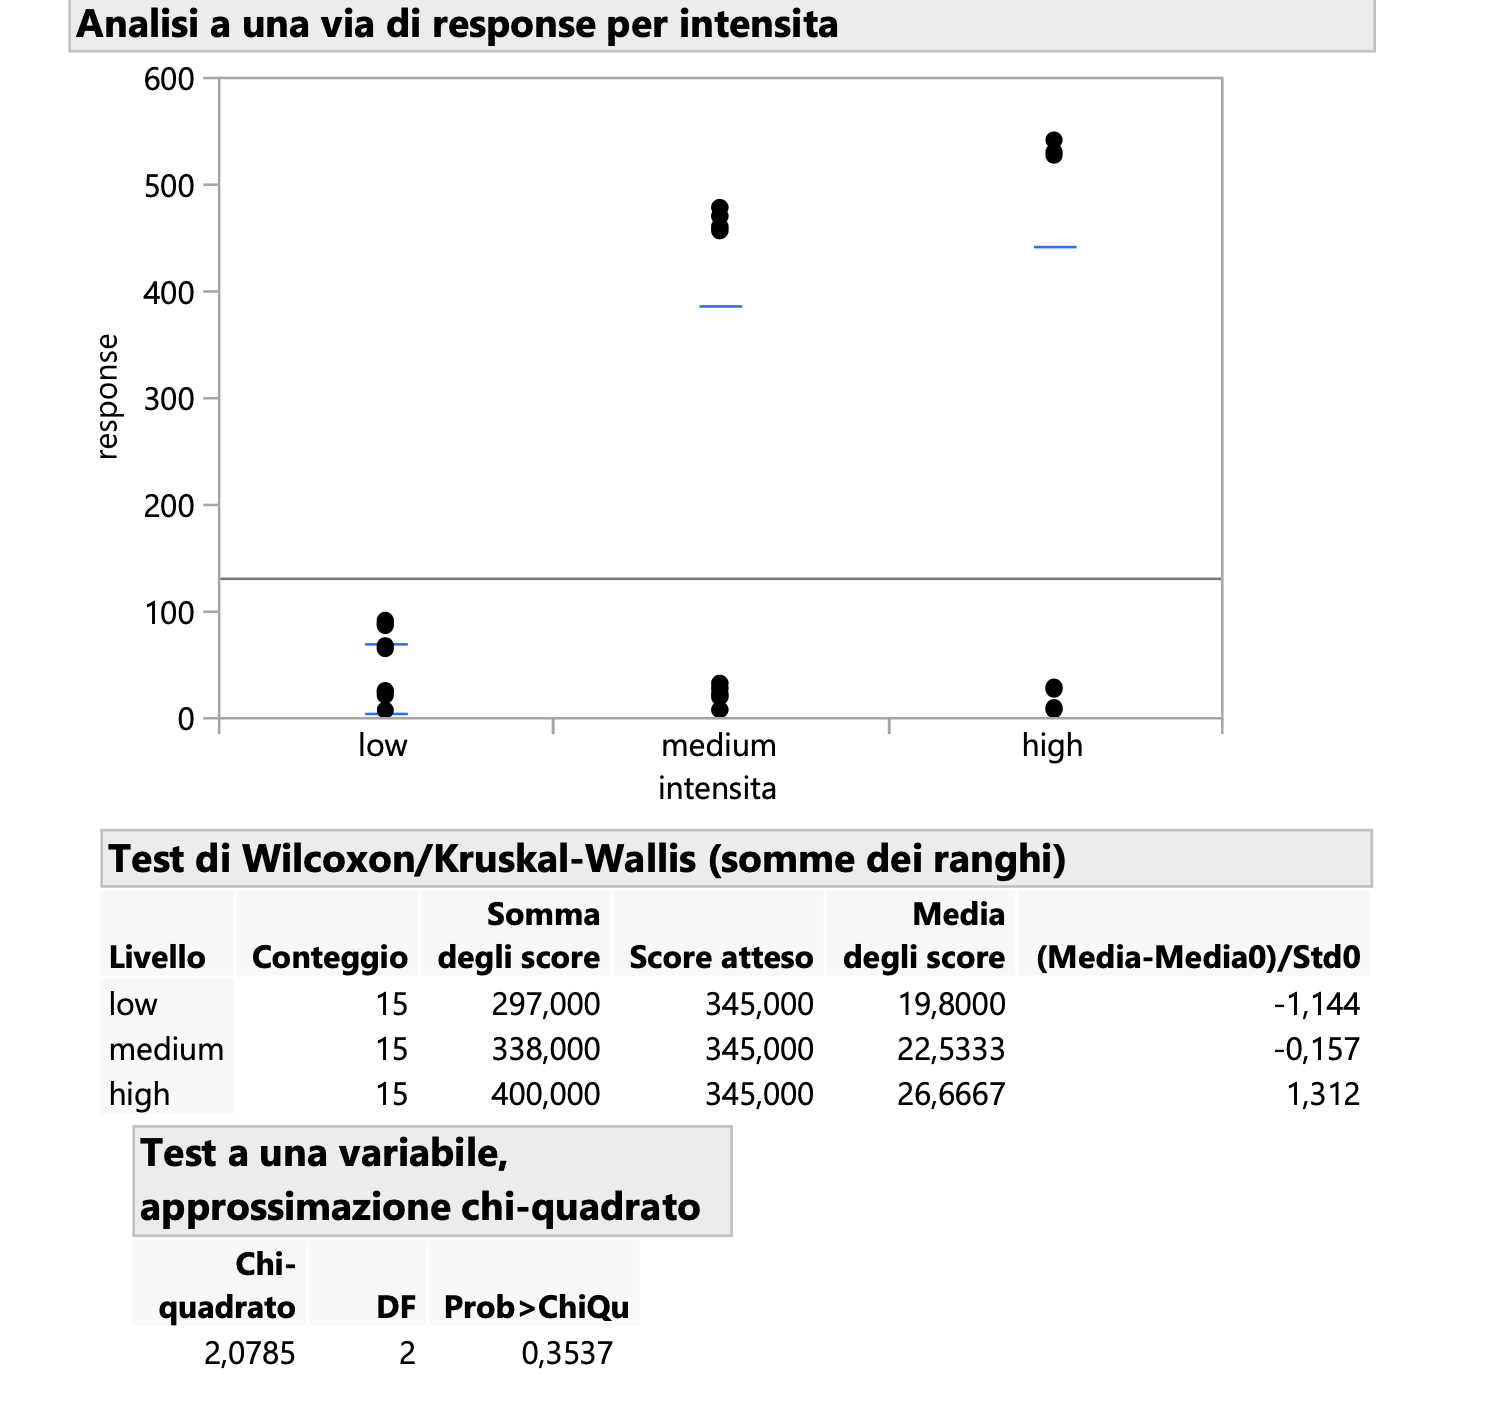
\includegraphics[scale=0.4]{img/chap_1/k_w_intensit.png}
    \caption{Kruskal-Wallis per l'intensità}
    \label{fig:k_w_int}
\end{figure}
\begin{figure}[H]
    \centering
    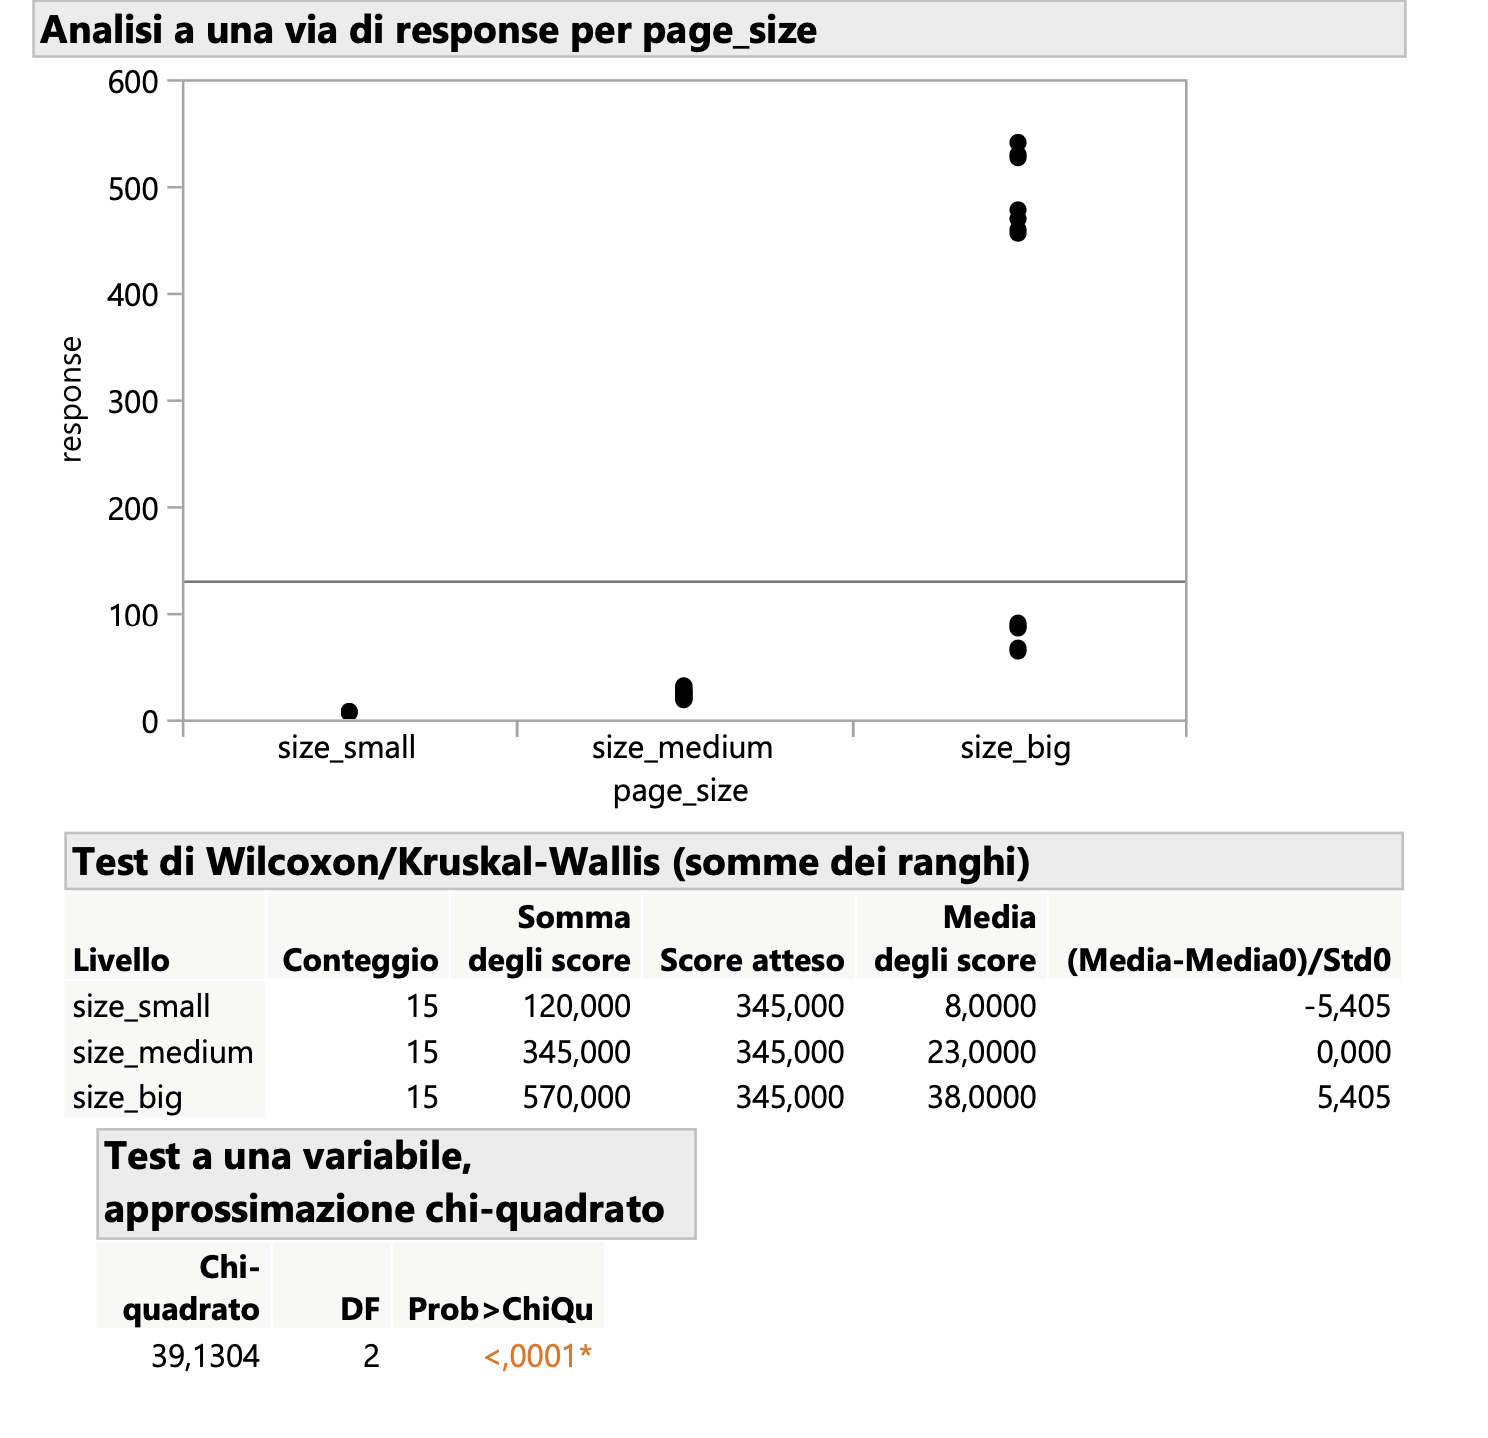
\includegraphics[scale=0.4]{img/chap_1/k_w_pageSize.png}
    \caption{Kruskal-Wallis per page\_size}
    \label{fig:k_w_ps}
\end{figure}
\noindent
Come si può notare dalla figura \ref{fig:k_w_int} il valore di ChiQuadro è molto alto non riuscendo a rigettare l'ipotesi nulla, riportando una non significatività del fattore, diverso invece è per \textit{page\_size} che dalle analisi che è possibile osservare dalla figura \ref{fig:k_w_ps} risulta essere significativo.\\
Dunque in definitiva avremo che \textit{page\_size} è un fattore importante e significativo mentre l'\textit{intensità} non è significativa ed è poco importante.\\ 


  